\documentclass[12pt]{article} 
\usepackage[margin=2cm]{geometry} 
\usepackage{psfrag} 
\usepackage{graphicx} 
\usepackage{epstopdf} 
\usepackage{longtable,booktabs} 
\usepackage{amsmath,amsfonts} 
\usepackage{breqn} 
\usepackage{float,morefloats,caption} 
\begin{document} 
% TeX eps-loader file generated by mode_check.m (Dynare).
% 27-Jul-2025 18:12:55
 
\begin{figure}[H]
\centering 
\includegraphics[width=0.80\textwidth]{SU_util/graphs/SU_util_CheckPlots1}
\caption{Check plots.}\label{Fig:CheckPlots:1}
\end{figure}
 
\begin{figure}[H]
\centering 
\includegraphics[width=0.80\textwidth]{SU_util/graphs/SU_util_CheckPlots2}
\caption{Check plots.}\label{Fig:CheckPlots:2}
\end{figure}
 
 
% 27-Jul-2025 18:13:31, created by mcmc_diagnostics.m 
 
\begin{center}
\begin{longtable}{lcc} 
\caption{MCMC Inefficiency factors per block}\\
 \label{Table:MCMC_inefficiency_factors}\\
\toprule 
$Parameter            $	 & 	 $     Block~1$	 & 	 $     Block~2$\\
\midrule \endfirsthead 
\caption{(continued)}\\
 \toprule \\ 
$Parameter            $	 & 	 $     Block~1$	 & 	 $     Block~2$\\
\midrule \endhead 
\midrule \multicolumn{3}{r}{(Continued on next page)} \\ \bottomrule \endfoot 
\bottomrule \endlastfoot 
$ \sigma_{{e_g}}      $	 & 	     555.483	 & 	     559.562 \\ 
$ \sigma_{{e_{ZI}}}   $	 & 	     303.552	 & 	     310.181 \\ 
$ \sigma_{{e_Z}}      $	 & 	     237.682	 & 	     277.491 \\ 
$ \sigma_{{e_N}}      $	 & 	     490.432	 & 	     508.176 \\ 
$ \sigma_{{e_D}}      $	 & 	     330.313	 & 	     347.109 \\ 
$ (\phi)              $	 & 	     743.460	 & 	     745.255 \\ 
$ (\eta)              $	 & 	     745.602	 & 	     743.083 \\ 
$ {\rho_g}            $	 & 	     740.614	 & 	     743.790 \\ 
$ {\rho_Z}            $	 & 	     684.882	 & 	     721.195 \\ 
$ {\rho_{ZI}}         $	 & 	     396.274	 & 	     635.785 \\ 
$ {\rho_N}            $	 & 	     730.380	 & 	     731.053 \\ 
$ {\rho_D}            $	 & 	     739.091	 & 	     742.063 \\ 
\end{longtable}
 \end{center}
% End of TeX file.
 
% TeX eps-loader file generated by McmcDiagnostics.m (Dynare).
% 30-Sep-2024 16:42:06
 
\begin{figure}[H]
\centering 
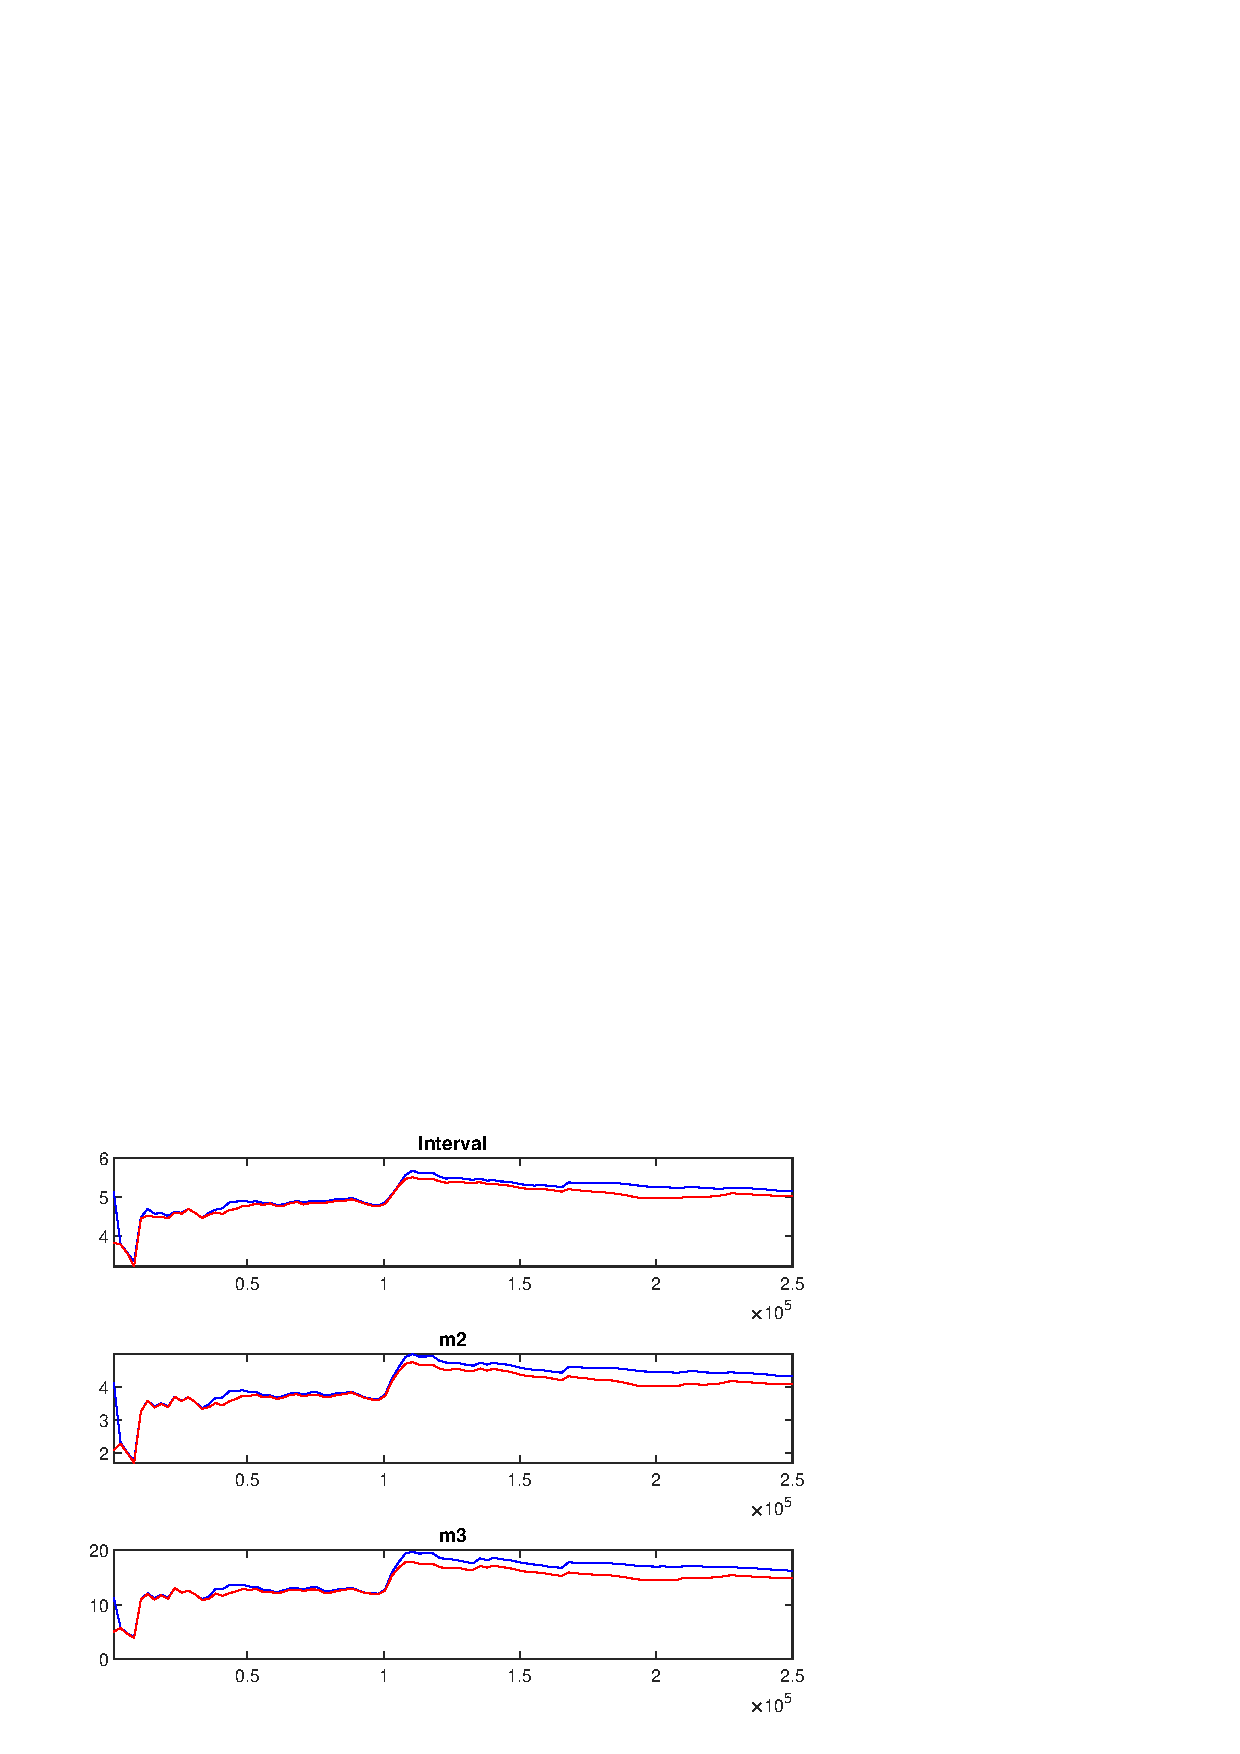
\includegraphics[width=0.8\textwidth]{BRS_util/Output/BRS_util_mdiag}
\caption{Multivariate convergence diagnostics for the Metropolis-Hastings.
The first, second and third rows are respectively the criteria based on
the eighty percent interval, the second and third moments. The different 
parameters are aggregated using the posterior kernel.}\label{Fig:MultivariateDiagnostics}
\end{figure}

% End Of TeX file. 
% TeX-table generated by Dynare.
% RESULTS FROM METROPOLIS HASTINGS (parameters)
% 30-Sep-2024 16:42:11 
 
\begin{center}
\begin{longtable}{llcccccc} 
\caption{Results from Metropolis-Hastings (parameters)}
 \label{Table:MHPosterior:1}\\
\toprule 
  & \multicolumn{3}{c}{Prior}  &  \multicolumn{4}{c}{Posterior} \\
  \cmidrule(r{.75em}){2-4} \cmidrule(r{.75em}){5-8}
  & Dist. & Mean  & Stdev. & Mean & Stdev. & HPD inf & HPD sup\\
\midrule \endfirsthead 
\caption{(continued)}\\\toprule 
  & \multicolumn{3}{c}{Prior}  &  \multicolumn{4}{c}{Posterior} \\
  \cmidrule(r{.75em}){2-4} \cmidrule(r{.75em}){5-8}
  & Dist. & Mean  & Stdev. & Mean & Stdev. & HPD inf & HPD sup\\
\midrule \endhead 
\bottomrule \multicolumn{8}{r}{(Continued on next page)} \endfoot 
\bottomrule \endlastfoot 
$(\phi)$ & beta &   0.320 & 0.2000 &   0.883& 0.0137 &  0.8628 &  0.9059 \\ 
$(\eta)$ & gamm &   0.200 & 0.1500 &   1.874& 0.0134 &  1.8575 &  1.8985 \\ 
${\rho_g}$ & beta &   0.100 & 0.0500 &   0.228& 0.0067 &  0.2199 &  0.2399 \\ 
${\rho_Z}$ & beta &   0.600 & 0.2000 &   0.972& 0.0039 &  0.9649 &  0.9770 \\ 
${\rho_{ZI}}$ & beta &   0.600 & 0.2000 &   0.999& 0.0011 &  0.9976 &  1.0000 \\ 
${\rho_N}$ & beta &   0.600 & 0.2000 &   0.979& 0.0054 &  0.9708 &  0.9883 \\ 
${\rho_D}$ & beta &   0.600 & 0.2000 &   0.928& 0.0090 &  0.9142 &  0.9408 \\ 
\end{longtable}
 \end{center}
% End of TeX file.
 
% TeX-table generated by Dynare.
% RESULTS FROM METROPOLIS HASTINGS (standard deviation of structural shocks)
% 30-Sep-2024 16:42:16 
 
\begin{center}
\begin{longtable}{llcccccc} 
\caption{Results from Metropolis-Hastings (standard deviation of structural shocks)}
 \label{Table:MHPosterior:2}\\
\toprule 
  & \multicolumn{3}{c}{Prior}  &  \multicolumn{4}{c}{Posterior} \\
  \cmidrule(r{.75em}){2-4} \cmidrule(r{.75em}){5-8}
  & Dist. & Mean  & Stdev. & Mean & Stdev. & HPD inf & HPD sup\\
\midrule \endfirsthead 
\caption{(continued)}\\\toprule 
  & \multicolumn{3}{c}{Prior}  &  \multicolumn{4}{c}{Posterior} \\
  \cmidrule(r{.75em}){2-4} \cmidrule(r{.75em}){5-8}
  & Dist. & Mean  & Stdev. & Mean & Stdev. & HPD inf & HPD sup\\
\midrule \endhead 
\bottomrule \multicolumn{8}{r}{(Continued on next page)} \endfoot 
\bottomrule \endlastfoot 
${e_g}$ & invg &   0.010 & 0.1000 &   0.017& 0.0007 &  0.0153 &  0.0177 \\ 
${e_{ZI}}$ & invg &   0.010 & 0.1000 &   0.008& 0.0004 &  0.0073 &  0.0086 \\ 
${e_Z}$ & invg &   0.010 & 0.1000 &   0.001& 0.0001 &  0.0008 &  0.0010 \\ 
${e_N}$ & invg &   0.010 & 0.1000 &   0.014& 0.0007 &  0.0127 &  0.0148 \\ 
${e_D}$ & invg &   0.010 & 0.1000 &   0.007& 0.0004 &  0.0068 &  0.0081 \\ 
\end{longtable}
 \end{center}
% End of TeX file.
 
% TeX-table generated by dynare_estimation (Dynare).
% RESULTS FROM POSTERIOR MAXIMIZATION (parameters)
% 30-Sep-2024 16:41:25 
 
\begin{center}
\begin{longtable}{llcccc} 
\caption{Results from posterior maximization (parameters)}\\
 \label{Table:Posterior:1}\\
\toprule 
  & \multicolumn{3}{c}{Prior}  &  \multicolumn{2}{c}{Posterior} \\
  \cmidrule(r{.75em}){2-4} \cmidrule(r{.75em}){5-6}
  & Dist. & Mean  & Stdev & Mode & Stdev \\ 
\midrule \endfirsthead 
\caption{(continued)}\\
 \bottomrule 
  & \multicolumn{3}{c}{Prior}  &  \multicolumn{2}{c}{Posterior} \\
  \cmidrule(r{.75em}){2-4} \cmidrule(r{.75em}){5-6}
  & Dist. & Mean  & Stdev & Mode & Stdev \\ 
\midrule \endhead 
\bottomrule \multicolumn{6}{r}{(Continued on next page)}\endfoot 
\bottomrule\endlastfoot 
$(\phi)$ & beta &   0.320 & 0.2000 &   0.8755 &     NaN \\ 
$(\eta)$ & gamm &   0.200 & 0.1500 &   1.8840 &     NaN \\ 
${\rho_g}$ & beta &   0.100 & 0.0500 &   0.2209 &     NaN \\ 
${\rho_Z}$ & beta &   0.600 & 0.2000 &   0.9709 &     NaN \\ 
${\rho_{ZI}}$ & beta &   0.600 & 0.2000 &   0.9994 &     NaN \\ 
${\rho_N}$ & beta &   0.600 & 0.2000 &   0.9816 &     NaN \\ 
${\rho_D}$ & beta &   0.600 & 0.2000 &   0.9275 &     NaN \\ 
\end{longtable}
 \end{center}
% End of TeX file.
 
% TeX-table generated by dynare_estimation (Dynare).
% RESULTS FROM POSTERIOR MAXIMIZATION (standard deviation of structural shocks)
% 30-Sep-2024 16:41:25 
 
\begin{center}
\begin{longtable}{llcccc} 
\caption{Results from posterior maximization (standard deviation of structural shocks)}\\
 \label{Table:Posterior:2}\\
\toprule 
  & \multicolumn{3}{c}{Prior}  &  \multicolumn{2}{c}{Posterior} \\
  \cmidrule(r{.75em}){2-4} \cmidrule(r{.75em}){5-6}
  & Dist. & Mean  & Stdev & Mode & Stdev \\ 
\midrule \endfirsthead 
\caption{(continued)}\\
 \bottomrule 
  & \multicolumn{3}{c}{Prior}  &  \multicolumn{2}{c}{Posterior} \\
  \cmidrule(r{.75em}){2-4} \cmidrule(r{.75em}){5-6}
  & Dist. & Mean  & Stdev & Mode & Stdev \\ 
\midrule \endhead 
\bottomrule \multicolumn{6}{r}{(Continued on next page)}\endfoot 
\bottomrule\endlastfoot 
${e_g}$ & invg &   0.010 & 0.1000 &   0.0165 &     NaN \\ 
${e_{ZI}}$ & invg &   0.010 & 0.1000 &   0.0079 &     NaN \\ 
${e_Z}$ & invg &   0.010 & 0.1000 &   0.0009 &     NaN \\ 
${e_N}$ & invg &   0.010 & 0.1000 &   0.0136 &     NaN \\ 
${e_D}$ & invg &   0.010 & 0.1000 &   0.0074 &     NaN \\ 
\end{longtable}
 \end{center}
% End of TeX file.
 
% TeX eps-loader file generated by plot_priors.m (Dynare).
% 30-Sep-2024 16:41:17
 
\begin{figure}[H]
\centering
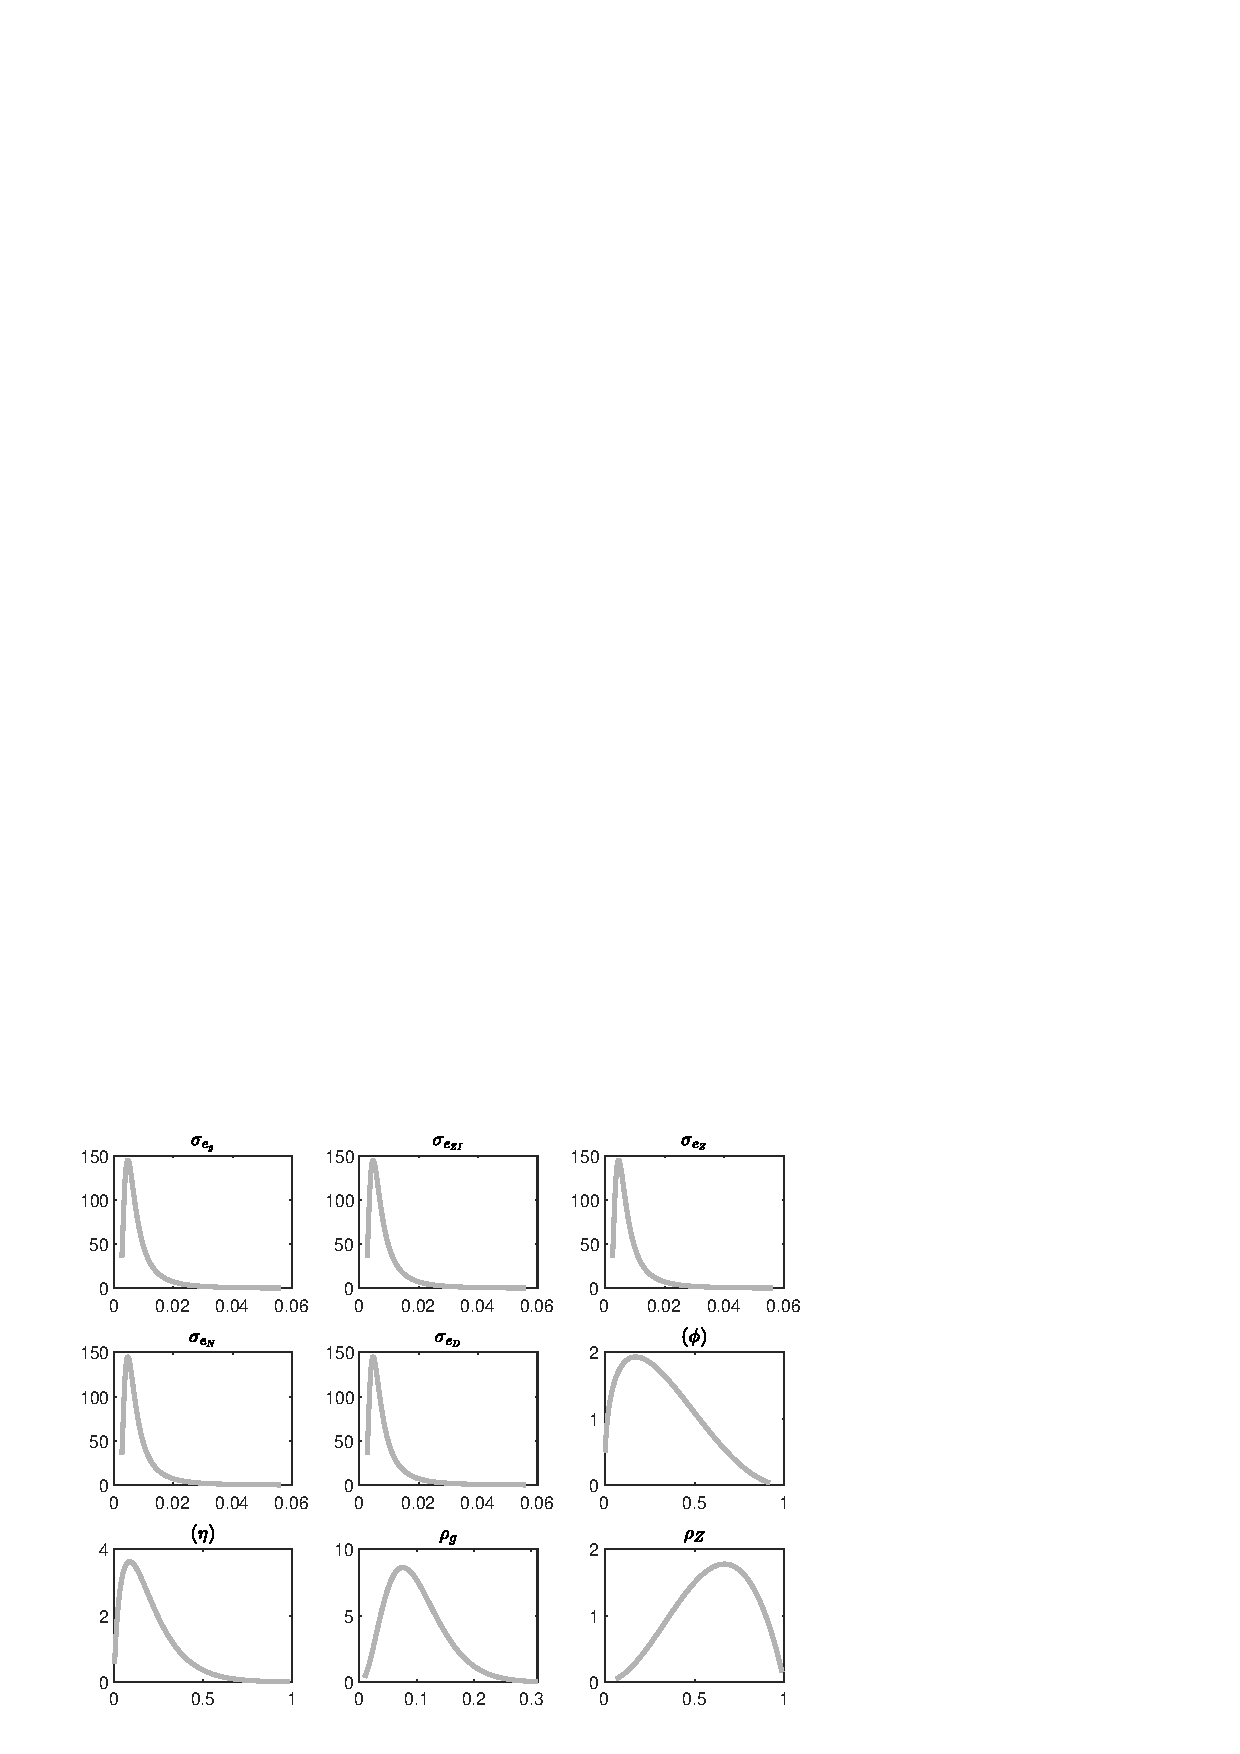
\includegraphics[width=0.80\textwidth]{BRS_util/graphs/BRS_util_Priors1}
\caption{Priors.}\label{Fig:Priors:1}
\end{figure}
\begin{figure}[H]
\centering
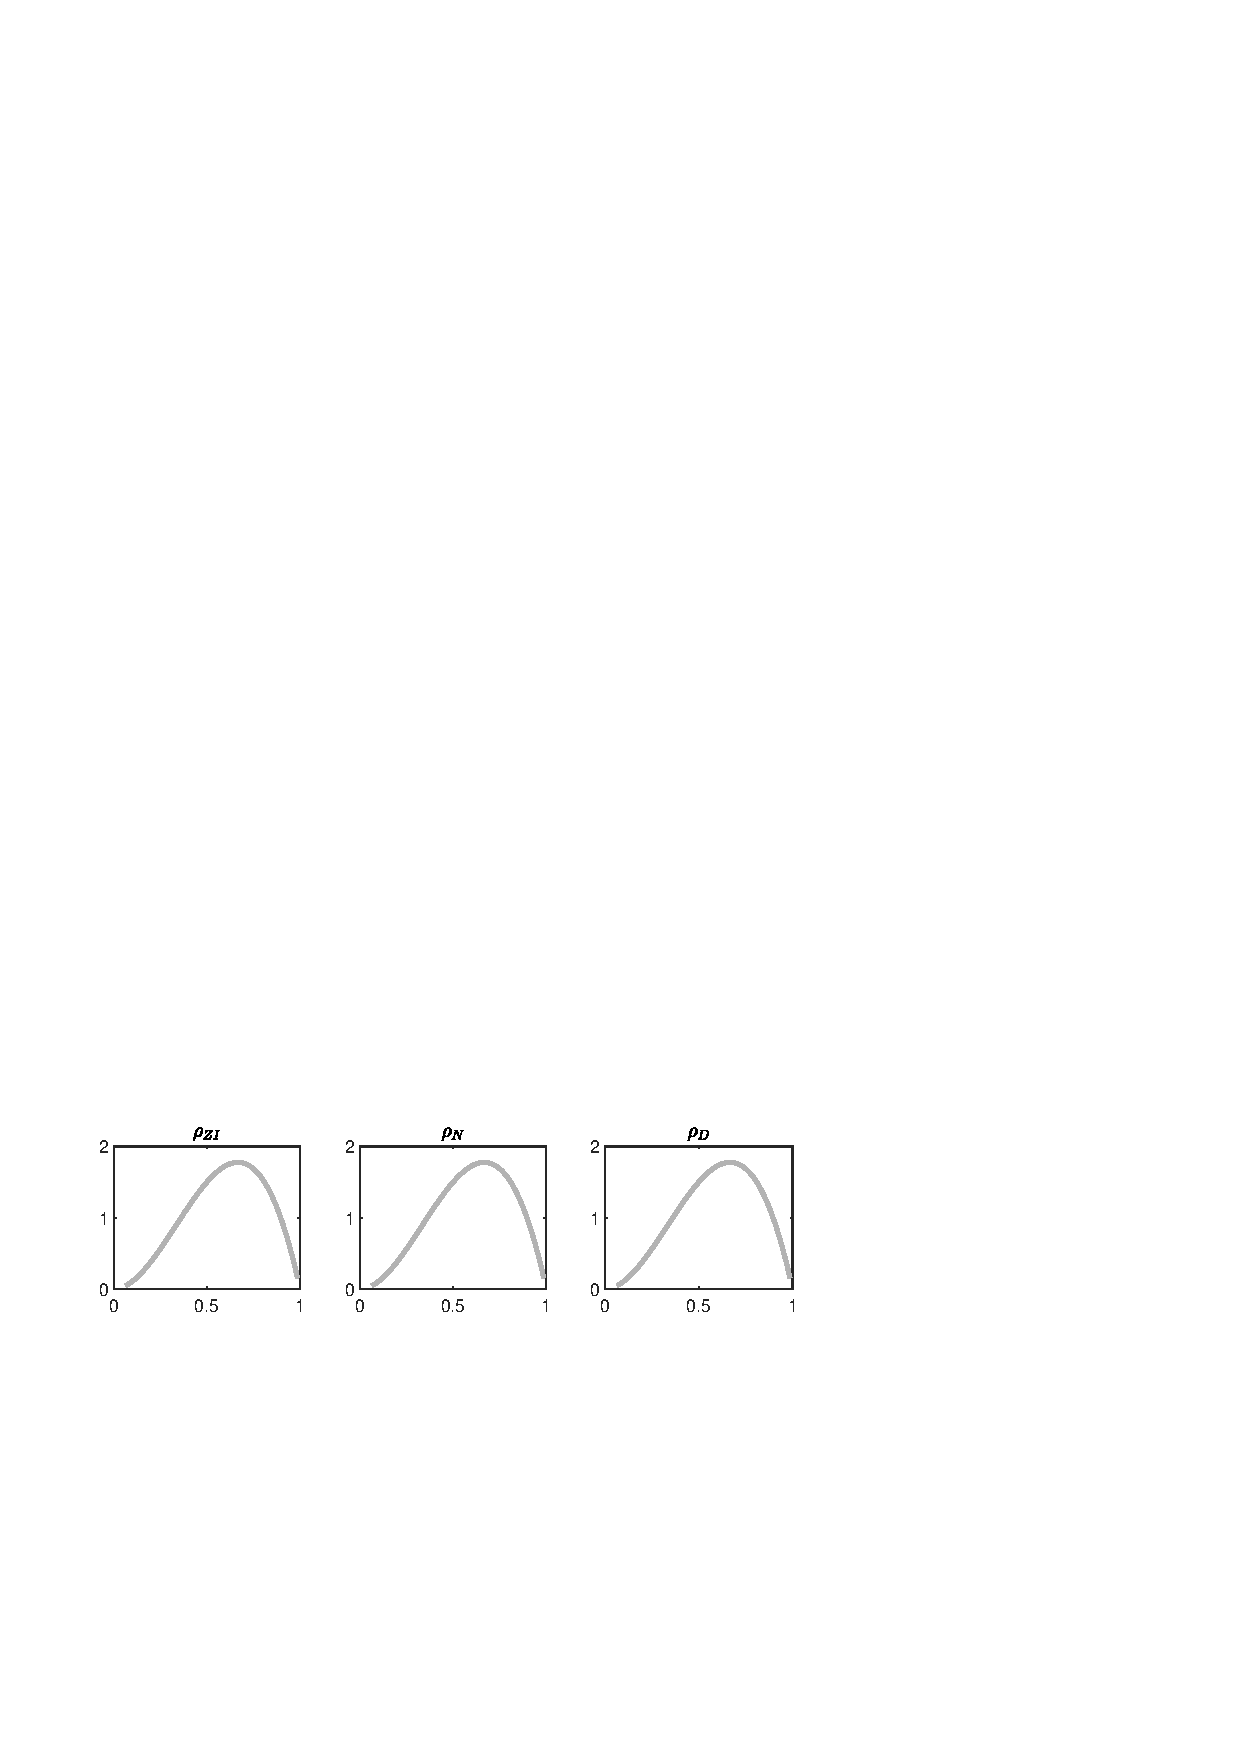
\includegraphics[width=0.80\textwidth]{BRS_util/graphs/BRS_util_Priors2}
\caption{Priors.}\label{Fig:Priors:2}
\end{figure}
 
% End of TeX file.
 
% TeX eps-loader file generated by PlotPosteriorDistributions.m (Dynare).
% 27-Jul-2025 18:14:06
 
\begin{figure}[H]
\centering
\includegraphics[width=0.80\textwidth]{SU_util/graphs/SU_util_PriorsAndPosteriors1}
\caption{Priors and posteriors.}\label{Fig:PriorsAndPosteriors:1}
\end{figure}
 
\begin{figure}[H]
\centering
\includegraphics[width=0.80\textwidth]{SU_util/graphs/SU_util_PriorsAndPosteriors2}
\caption{Priors and posteriors.}\label{Fig:PriorsAndPosteriors:2}
\end{figure}
 
% End of TeX file.
 
% TeX eps-loader file generated by mcmc_diagnostics.m (Dynare).
% 27-Jul-2025 18:13:33
 
\begin{figure}[H]
\centering 
\includegraphics[width=0.80\textwidth]{SU_util/graphs/SU_util_udiag1}
\caption{Univariate convergence diagnostics for the Metropolis-Hastings.
The first, second and third columns are respectively the criteria based on
the eighty percent interval, the second and third moments.}\label{Fig:UnivariateDiagnostics:1}
\end{figure}

\begin{figure}[H]
\centering 
\includegraphics[width=0.80\textwidth]{SU_util/graphs/SU_util_udiag2}
\caption{Univariate convergence diagnostics for the Metropolis-Hastings.
The first, second and third columns are respectively the criteria based on
the eighty percent interval, the second and third moments.}\label{Fig:UnivariateDiagnostics:2}
\end{figure}

\begin{figure}[H]
\centering 
\includegraphics[width=0.80\textwidth]{SU_util/graphs/SU_util_udiag3}
\caption{Univariate convergence diagnostics for the Metropolis-Hastings.
The first, second and third columns are respectively the criteria based on
the eighty percent interval, the second and third moments.}\label{Fig:UnivariateDiagnostics:3}
\end{figure}

\begin{figure}[H]
\centering 
\includegraphics[width=0.80\textwidth]{SU_util/graphs/SU_util_udiag4}
\caption{Univariate convergence diagnostics for the Metropolis-Hastings.
The first, second and third columns are respectively the criteria based on
the eighty percent interval, the second and third moments.}\label{Fig:UnivariateDiagnostics:4}
\end{figure}

 
% 27-Jul-2025 18:14:09, created by stoch_simul.m 
 
\begin{center}
\begin{longtable}{lccccc} 
\caption{MATRIX OF COVARIANCE OF EXOGENOUS SHOCKS}\\
 \label{Table:covar_ex_shocks}\\
\toprule 
$Variables  $	 & 	 $       {e_g}$	 & 	 $       {e_Z}$	 & 	 $    {e_{ZI}}$	 & 	 $       {e_N}$	 & 	 $       {e_D}$\\
\midrule \endfirsthead 
\caption{(continued)}\\
 \toprule \\ 
$Variables  $	 & 	 $       {e_g}$	 & 	 $       {e_Z}$	 & 	 $    {e_{ZI}}$	 & 	 $       {e_N}$	 & 	 $       {e_D}$\\
\midrule \endhead 
\midrule \multicolumn{6}{r}{(Continued on next page)} \\ \bottomrule \endfoot 
\bottomrule \endlastfoot 
${e_g}      $	 & 	    0.000273	 & 	    0.000000	 & 	    0.000000	 & 	    0.000000	 & 	    0.000000 \\ 
${e_Z}      $	 & 	    0.000000	 & 	    0.000001	 & 	    0.000000	 & 	    0.000000	 & 	    0.000000 \\ 
${e_{ZI}}   $	 & 	    0.000000	 & 	    0.000000	 & 	    0.000063	 & 	    0.000000	 & 	    0.000000 \\ 
${e_N}      $	 & 	    0.000000	 & 	    0.000000	 & 	    0.000000	 & 	    0.000189	 & 	    0.000000 \\ 
${e_D}      $	 & 	    0.000000	 & 	    0.000000	 & 	    0.000000	 & 	    0.000000	 & 	    0.000056 \\ 
\end{longtable}
 \end{center}
% End of TeX file.
 
% 16-Apr-2024 16:44:57, created by compute_moments_varendo.m 
 
\begin{center}
\begin{longtable}{lccccc} 
\caption{Posterior mean variance decomposition (in percent)}\\
 \label{Table:dsge_post_mean_var_decomp_uncond}\\
\toprule 
$           $	 & 	 $       {e_g}$	 & 	 $       {e_Z}$	 & 	 $    {e_{ZI}}$	 & 	 $       {e_N}$	 & 	 $       {e_D}$\\
\midrule \endfirsthead 
\caption{(continued)}\\
 \toprule \\ 
$           $	 & 	 $       {e_g}$	 & 	 $       {e_Z}$	 & 	 $    {e_{ZI}}$	 & 	 $       {e_N}$	 & 	 $       {e_D}$\\
\midrule \endhead 
\midrule \multicolumn{6}{r}{(Continued on next page)} \\ \bottomrule \endfoot 
\bottomrule \endlastfoot 
$Y\_obs     $	 & 	        0.97	 & 	       33.70	 & 	        3.11	 & 	        0.68	 & 	       61.55 \\ 
$Y\_N\_obs  $	 & 	       39.16	 & 	       15.23	 & 	        2.43	 & 	       16.64	 & 	       26.55 \\ 
$I\_obs     $	 & 	        0.23	 & 	       22.65	 & 	       11.66	 & 	        0.53	 & 	       64.93 \\ 
$p\_I\_obs  $	 & 	        0.01	 & 	       25.35	 & 	       61.92	 & 	        0.07	 & 	       12.66 \\ 
$C\_obs     $	 & 	        1.25	 & 	       46.52	 & 	        2.22	 & 	        0.62	 & 	       49.39 \\ 
$util\_obs  $	 & 	       36.24	 & 	       10.26	 & 	        0.58	 & 	        0.21	 & 	       52.72 \\ 
\end{longtable}
 \end{center}
% End of TeX file.
 
% 27-Jul-2025 18:13:32, created by mcmc_diagnostics.m 
 
\begin{center}
\begin{longtable}{lcccccc} 
\caption{Geweke (1992) Convergence Tests, based on means of draws 75000 to 110000 vs 162500 to 250000 for chain 1. p-values are for $\chi^2$-test for equality of means.}\\
 \label{Table:geweke_block_1}\\
\toprule 
 & \multicolumn{2}{c}{Posterior} & \multicolumn{4}{c}{p-values} \\
\cmidrule(r{.75em}){2-3} \cmidrule(r{.75em}){4-7}
$Parameter            $	 & 	 $            Mean$	 & 	 $             Std$	 & 	 $      No\ Taper$	 & 	 $   4\%\ Taper$	 & 	 $   8\%\ Taper$	 & 	 $  15\%\ Taper$\\
\midrule \endfirsthead 
\caption{(continued)}\\
 \toprule \\ 
 & \multicolumn{2}{c}{Posterior} & \multicolumn{4}{c}{p-values} \\
\cmidrule(r{.75em}){2-3} \cmidrule(r{.75em}){4-7}
$Parameter            $	 & 	 $            Mean$	 & 	 $             Std$	 & 	 $      No\ Taper$	 & 	 $   4\%\ Taper$	 & 	 $   8\%\ Taper$	 & 	 $  15\%\ Taper$\\
\midrule \endhead 
\midrule \multicolumn{7}{r}{(Continued on next page)} \\ \bottomrule \endfoot 
\bottomrule \endlastfoot 
$ \sigma_{{e_g}}      $	 & 	          0.0165	 & 	          0.0008	 & 	          0.0003	 & 	          0.9065	 & 	          0.9179	 & 	          0.9203 \\ 
$ \sigma_{{e_{ZI}}}   $	 & 	          0.0080	 & 	          0.0004	 & 	          0.0000	 & 	          0.0466	 & 	          0.0642	 & 	          0.0812 \\ 
$ \sigma_{{e_Z}}      $	 & 	          0.0010	 & 	          0.0001	 & 	          0.0000	 & 	          0.0299	 & 	          0.0626	 & 	          0.0692 \\ 
$ \sigma_{{e_N}}      $	 & 	          0.0137	 & 	          0.0006	 & 	          0.0000	 & 	          0.3337	 & 	          0.3780	 & 	          0.4144 \\ 
$ \sigma_{{e_D}}      $	 & 	          0.0075	 & 	          0.0004	 & 	          0.0000	 & 	          0.0009	 & 	          0.0068	 & 	          0.0221 \\ 
$ (\phi)              $	 & 	          0.8748	 & 	          0.0113	 & 	          0.0000	 & 	          0.0000	 & 	          0.0000	 & 	          0.0000 \\ 
$ (\eta)              $	 & 	          1.8680	 & 	          0.0107	 & 	          0.0000	 & 	          0.0000	 & 	          0.0001	 & 	          0.0036 \\ 
$ {\rho_g}            $	 & 	          0.2305	 & 	          0.0062	 & 	          0.0000	 & 	          0.0000	 & 	          0.0003	 & 	          0.0050 \\ 
$ {\rho_Z}            $	 & 	          0.9713	 & 	          0.0032	 & 	          0.0000	 & 	          0.1100	 & 	          0.1608	 & 	          0.1727 \\ 
$ {\rho_{ZI}}         $	 & 	          0.9989	 & 	          0.0008	 & 	          0.0000	 & 	          0.6958	 & 	          0.7165	 & 	          0.7361 \\ 
$ {\rho_N}            $	 & 	          0.9793	 & 	          0.0054	 & 	          0.0000	 & 	          0.1797	 & 	          0.2900	 & 	          0.3427 \\ 
$ {\rho_D}            $	 & 	          0.9310	 & 	          0.0075	 & 	          0.0000	 & 	          0.7220	 & 	          0.7953	 & 	          0.8412 \\ 
\end{longtable}
 \end{center}
% End of TeX file.
 
% 27-Jul-2025 18:13:33, created by mcmc_diagnostics.m 
 
\begin{center}
\begin{longtable}{lcccccc} 
\caption{Geweke (1992) Convergence Tests, based on means of draws 75000 to 110000 vs 162500 to 250000 for chain 2. p-values are for $\chi^2$-test for equality of means.}\\
 \label{Table:geweke_block_2}\\
\toprule 
 & \multicolumn{2}{c}{Posterior} & \multicolumn{4}{c}{p-values} \\
\cmidrule(r{.75em}){2-3} \cmidrule(r{.75em}){4-7}
$Parameter            $	 & 	 $            Mean$	 & 	 $             Std$	 & 	 $      No\ Taper$	 & 	 $   4\%\ Taper$	 & 	 $   8\%\ Taper$	 & 	 $  15\%\ Taper$\\
\midrule \endfirsthead 
\caption{(continued)}\\
 \toprule \\ 
 & \multicolumn{2}{c}{Posterior} & \multicolumn{4}{c}{p-values} \\
\cmidrule(r{.75em}){2-3} \cmidrule(r{.75em}){4-7}
$Parameter            $	 & 	 $            Mean$	 & 	 $             Std$	 & 	 $      No\ Taper$	 & 	 $   4\%\ Taper$	 & 	 $   8\%\ Taper$	 & 	 $  15\%\ Taper$\\
\midrule \endhead 
\midrule \multicolumn{7}{r}{(Continued on next page)} \\ \bottomrule \endfoot 
\bottomrule \endlastfoot 
$ \sigma_{{e_g}}      $	 & 	          0.0166	 & 	          0.0007	 & 	          0.0000	 & 	          0.4991	 & 	          0.5726	 & 	          0.5951 \\ 
$ \sigma_{{e_{ZI}}}   $	 & 	          0.0079	 & 	          0.0004	 & 	          0.0000	 & 	          0.6883	 & 	          0.7187	 & 	          0.7280 \\ 
$ \sigma_{{e_Z}}      $	 & 	          0.0009	 & 	          0.0001	 & 	          0.0000	 & 	          0.3230	 & 	          0.4561	 & 	          0.5622 \\ 
$ \sigma_{{e_N}}      $	 & 	          0.0138	 & 	          0.0006	 & 	          0.0626	 & 	          0.9460	 & 	          0.9489	 & 	          0.9473 \\ 
$ \sigma_{{e_D}}      $	 & 	          0.0075	 & 	          0.0004	 & 	          0.0000	 & 	          0.1641	 & 	          0.2665	 & 	          0.3795 \\ 
$ (\phi)              $	 & 	          0.8829	 & 	          0.0150	 & 	          0.0000	 & 	          0.0663	 & 	          0.1859	 & 	          0.3158 \\ 
$ (\eta)              $	 & 	          1.8828	 & 	          0.0078	 & 	          0.0000	 & 	          0.0000	 & 	          0.0007	 & 	          0.0097 \\ 
$ {\rho_g}            $	 & 	          0.2217	 & 	          0.0022	 & 	          0.0000	 & 	          0.0000	 & 	          0.0000	 & 	          0.0000 \\ 
$ {\rho_Z}            $	 & 	          0.9714	 & 	          0.0044	 & 	          0.0000	 & 	          0.0117	 & 	          0.0639	 & 	          0.1526 \\ 
$ {\rho_{ZI}}         $	 & 	          0.9988	 & 	          0.0012	 & 	          0.0000	 & 	          0.0113	 & 	          0.0629	 & 	          0.1478 \\ 
$ {\rho_N}            $	 & 	          0.9774	 & 	          0.0065	 & 	          0.0000	 & 	          0.0021	 & 	          0.0219	 & 	          0.0657 \\ 
$ {\rho_D}            $	 & 	          0.9244	 & 	          0.0081	 & 	          0.0000	 & 	          0.0000	 & 	          0.0000	 & 	          0.0000 \\ 
\end{longtable}
 \end{center}
% End of TeX file.
 
\begin{center}
\begin{longtable}{ccc}
\caption{Endogenous}\\%
\hline%
\multicolumn{1}{c}{\textbf{Variable}} &
\multicolumn{1}{c}{\textbf{\LaTeX}} &
\multicolumn{1}{c}{\textbf{Description}}\\%
\hline\hline%
\endfirsthead
\multicolumn{3}{c}{{\tablename} \thetable{} -- Continued}\\%
\hline%
\multicolumn{1}{c}{\textbf{Variable}} &
\multicolumn{1}{c}{\textbf{\LaTeX}} &
\multicolumn{1}{c}{\textbf{Description}}\\%
\hline\hline%
\endhead
\texttt{Y} & ${Y}$ & output\\
\texttt{C} & ${C}$ & consumption\\
\texttt{I} & ${I}$ & investment\\
\texttt{SR} & ${SR}$ & aggregate share-weighted Solow residual\\
\texttt{K} & ${K}$ & Capital\\
\texttt{K\_C} & ${K_C}$ & Capital:C\\
\texttt{K\_I} & ${K_I}$ & Capital:I\\
\texttt{N} & ${N}$ & Hours\\
\texttt{N\_C} & ${N_C}$ & Hours:C\\
\texttt{N\_I} & ${N_I}$ & Hours:I\\
\texttt{Z\_C} & ${Z_C}$ & Tech:C\\
\texttt{u\_ZI} & $u\_ZI$ & u\_ZI\\
\texttt{Z\_I} & ${Z_I}$ & Tech:I\\
\texttt{theta\_N} & ${\theta_N}$ & Labor disutility\\
\texttt{theta\_D} & ${\theta_D}$ & Shopping disutility\\
\texttt{R\_C} & ${R_C}$ & Capital rental rate:C\\
\texttt{R\_I} & ${R_I}$ & Capital rental rate:I\\
\texttt{W} & ${W}$ & Real wage\\
\texttt{D} & ${D}$ & Shopping effort\\
\texttt{D\_C} & ${D}$ & Shopping effort:C\\
\texttt{D\_I} & ${D}$ & Shopping effort:I\\
\texttt{Gam} & ${\Gamma}$ & Composite utility term\\
\texttt{p\_I} & ${p_I}$ & Relative investment price\\
\texttt{g} & ${g}$ & Output growth rate (labor-augmenting technology)\\
\texttt{util\_C} & $util\_C$ & util\_C\\
\texttt{util\_I} & $util\_I$ & util\_I\\
\texttt{util} & $util$ & util\\
\texttt{log\_Y} & $log\_Y$ & log\_Y\\
\texttt{log\_C} & $log\_C$ & log\_C\\
\texttt{log\_I} & $log\_I$ & log\_I\\
\texttt{log\_N} & $log\_N$ & log\_N\\
\texttt{log\_NC} & $log\_NC$ & log\_NC\\
\texttt{log\_NI} & $log\_NI$ & log\_NI\\
\texttt{log\_Y\_N} & $log\_Y\_N$ & log\_Y\_N\\
\texttt{log\_SR} & $log\_SR$ & log\_SR\\
\texttt{log\_D} & $log\_D$ & log\_D\\
\texttt{log\_p\_I} & $log\_p\_I$ & log\_p\_I\\
\texttt{log\_util} & $log\_util$ & log\_util\\
\texttt{log\_util\_C} & $log\_util\_C$ & log\_util\_C\\
\texttt{log\_util\_I} & $log\_util\_I$ & log\_util\_I\\
\texttt{C\_obs} & $C\_obs$ & C\_obs\\
\texttt{I\_obs} & $I\_obs$ & I\_obs\\
\texttt{Y\_obs} & $Y\_obs$ & Y\_obs\\
\texttt{Y\_N\_obs} & $Y\_N\_obs$ & Y\_N\_obs\\
\texttt{SR\_obs} & $SR\_obs$ & SR\_obs\\
\texttt{p\_I\_obs} & $p\_I\_obs$ & p\_I\_obs\\
\texttt{NC\_obs} & $NC\_obs$ & NC\_obs\\
\texttt{NI\_obs} & $NI\_obs$ & NI\_obs\\
\texttt{N\_obs} & $N\_obs$ & N\_obs\\
\texttt{D\_obs} & $D\_obs$ & D\_obs\\
\texttt{util\_obs} & $util\_obs$ & util\_obs\\
\texttt{util\_C\_obs} & $util\_C\_obs$ & util\_C\_obs\\
\texttt{util\_I\_obs} & $util\_I\_obs$ & util\_I\_obs\\
\hline%
\end{longtable}
\end{center}
\begin{center}
\begin{longtable}{ccc}
\caption{Exogenous}\\%
\hline%
\multicolumn{1}{c}{\textbf{Variable}} &
\multicolumn{1}{c}{\textbf{\LaTeX}} &
\multicolumn{1}{c}{\textbf{Description}}\\%
\hline\hline%
\endfirsthead
\multicolumn{3}{c}{{\tablename} \thetable{} -- Continued}\\%
\hline%
\multicolumn{1}{c}{\textbf{Variable}} &
\multicolumn{1}{c}{\textbf{\LaTeX}} &
\multicolumn{1}{c}{\textbf{Description}}\\%
\hline\hline%
\endhead
\texttt{e\_g} & ${e_g}$ & TFP shock\\
\texttt{e\_Z} & ${e_Z}$ & TFP shock\\
\texttt{e\_ZI} & ${e_{ZI}}$ & Investment-specific tech shock\\
\texttt{e\_N} & ${e_N}$ & Labor supply shock\\
\texttt{e\_D} & ${e_D}$ & Shopping disutility shock\\
\hline%
\end{longtable}
\end{center}
\begin{center}
\begin{longtable}{ccc}
\caption{Parameters}\\%
\hline%
\multicolumn{1}{c}{\textbf{Variable}} &
\multicolumn{1}{c}{\textbf{\LaTeX}} &
\multicolumn{1}{c}{\textbf{Description}}\\%
\hline\hline%
\endfirsthead
\multicolumn{3}{c}{{\tablename} \thetable{} -- Continued}\\%
\hline%
\multicolumn{1}{c}{\textbf{Variable}} &
\multicolumn{1}{c}{\textbf{\LaTeX}} &
\multicolumn{1}{c}{\textbf{Description}}\\%
\hline\hline%
\endhead
\texttt{sigma} & ${\sigma}$ & Risk aversion\\
\texttt{beta} & ${\beta}$ & Discount factor\\
\texttt{g\_bar} & ${\overline{g}}$ & Quarterly growth rate\\
\texttt{nu} & $(\nu)$ & Frisch elasticity\\
\texttt{I\_Y} & $(I_Y)$ & Investment-output ratio\\
\texttt{K\_Y} & $(K_Y)$ & Capital-output ratio (quarterly)\\
\texttt{labor\_share} & $(labor share)$ & Labor share\\
\texttt{phi} & $(\phi)$ & Shopping matching function elasticity\\
\texttt{eta} & $(\eta)$ & Shopping disutility\\
\texttt{Psi} & $(\Psi)$ & Matching utilization\\
\texttt{rho\_g} & ${\rho_g}$ & persistence shock to labor-augmenting technology growth rate\\
\texttt{rho\_Z} & ${\rho_Z}$ & persistence TFP shock\\
\texttt{rho\_ZI} & ${\rho_{ZI}}$ & persistence I-specific shock\\
\texttt{rho\_N} & ${\rho_N}$ & persistence labor supply shock\\
\texttt{rho\_D} & ${\rho_D}$ & persistence shopping effort shock\\
\texttt{p\_I\_ss} & $p\_I\_ss$ & p\_I\_ss\\
\texttt{N\_ss} & $N\_ss$ & N\_ss\\
\hline%
\end{longtable}
\end{center}
 
\begin{center}
\begin{longtable}{ccc}
\caption{Parameter Values}\\%
\toprule%
\multicolumn{1}{c}{\textbf{Parameter}} &
\multicolumn{1}{c}{\textbf{Value}} &
 \multicolumn{1}{c}{\textbf{Description}}\\%
\midrule%
\endfirsthead
\multicolumn{3}{c}{{\tablename} \thetable{} -- Continued}\\%
\midrule%
\multicolumn{1}{c}{\textbf{Parameter}} &
\multicolumn{1}{c}{\textbf{Value}} &
  \multicolumn{1}{c}{\textbf{Description}}\\%
\midrule%
\endhead
${\sigma}$ 	 & 	 2.000 	 & 	 Risk aversion\\
${\beta}$ 	 & 	 0.990 	 & 	 Discount factor\\
${\overline{g}}$ 	 & 	 0.004 	 & 	 Quarterly growth rate\\
$(\nu)$ 	 & 	 0.720 	 & 	 Frisch elasticity\\
$(I_Y)$ 	 & 	 0.200 	 & 	 Investment-output ratio\\
$(K_Y)$ 	 & 	 11.000 	 & 	 Capital-output ratio (quarterly)\\
$(labor share)$ 	 & 	 0.670 	 & 	 Labor share\\
$(\phi)$ 	 & 	 0.883 	 & 	 Shopping matching function elasticity\\
$(\eta)$ 	 & 	 1.874 	 & 	 Shopping disutility\\
$(\Psi)$ 	 & 	 0.810 	 & 	 Matching utilization\\
${\rho_g}$ 	 & 	 0.228 	 & 	 persistence shock to labor-augmenting technology growth rate\\
${\rho_Z}$ 	 & 	 0.972 	 & 	 persistence TFP shock\\
${\rho_{ZI}}$ 	 & 	 0.999 	 & 	 persistence I-specific shock\\
${\rho_N}$ 	 & 	 0.979 	 & 	 persistence labor supply shock\\
${\rho_D}$ 	 & 	 0.928 	 & 	 persistence shopping effort shock\\
$p\_I\_ss$ 	 & 	 1.000 	 & 	 p\_I\_ss\\
$N\_ss$ 	 & 	 0.300 	 & 	 N\_ss\\
\bottomrule%
\end{longtable}
\end{center}
 
% TeX-table generated by Dynare write_latex_prior_table.m.
% Prior Information
% 27-Jul-2025 18:14:09 
 
\begin{center}
\begin{longtable}{lcccccccc} 
\caption{Prior information (parameters)}\\
 \label{Table:Prior}\\
\toprule%
  &  &  &  &  & \multicolumn{2}{c}{Bounds} & \multicolumn{2}{c}{90\% HPDI} \\ 
  \cmidrule(r{.75em}){6-7} \cmidrule(r{.75em}){8-9}
  & Distribution & Mean & Mode & Std.dev. & Lower & Upper & Lower & Upper  \\ 
\midrule
\endfirsthead
\caption{(continued)}\\
 \toprule%
  &  &  &  &  & \multicolumn{2}{c}{Bounds} & \multicolumn{2}{c}{90\% HPDI} \\ 
  \cmidrule(r{.75em}){6-7} \cmidrule(r{.75em}){8-9}
  & Distribution & Mean & Mode & Std.dev. & Lower & Upper & Lower & Upper  \\ 
\midrule
\endhead
\midrule
\multicolumn{9}{r}{(Continued on next page)} \\ 
\bottomrule
\endfoot
\bottomrule
\endlastfoot
$ \sigma_{{e_g}} $ & Inv. Gamma & 0.0100 & 0.0046 & 0.1000 & 0.0000 & $\infty$ & 0.0033 & 0.0249 \\ 
$ \sigma_{{e_{ZI}}} $ & Inv. Gamma & 0.0100 & 0.0046 & 0.1000 & 0.0000 & $\infty$ & 0.0033 & 0.0249 \\ 
$ \sigma_{{e_Z}} $ & Inv. Gamma & 0.0100 & 0.0046 & 0.1000 & 0.0000 & $\infty$ & 0.0033 & 0.0249 \\ 
$ \sigma_{{e_N}} $ & Inv. Gamma & 0.0100 & 0.0046 & 0.1000 & 0.0000 & $\infty$ & 0.0033 & 0.0249 \\ 
$ \sigma_{{e_D}} $ & Inv. Gamma & 0.0100 & 0.0046 & 0.1000 & 0.0000 & $\infty$ & 0.0033 & 0.0249 \\ 
$ (\phi) $ & Beta & 0.3200 & 0.1725 & 0.2000 & 0.0000 & 1.0000 & 0.0462 & 0.6925 \\ 
$ (\eta) $ & Gamma & 0.2000 & 0.0875 & 0.1500 & 0.0000 & $\infty$ & 0.0304 & 0.4926 \\ 
$ {\rho_g} $ & Beta & 0.1000 & 0.0758 & 0.0500 & 0.0000 & 1.0000 & 0.0326 & 0.1935 \\ 
$ {\rho_Z} $ & Beta & 0.6000 & 0.6667 & 0.2000 & 0.0000 & 1.0000 & 0.2486 & 0.9024 \\ 
$ {\rho_{ZI}} $ & Beta & 0.6000 & 0.6667 & 0.2000 & 0.0000 & 1.0000 & 0.2486 & 0.9024 \\ 
$ {\rho_N} $ & Beta & 0.6000 & 0.6667 & 0.2000 & 0.0000 & 1.0000 & 0.2486 & 0.9024 \\ 
$ {\rho_D} $ & Beta & 0.6000 & 0.6667 & 0.2000 & 0.0000 & 1.0000 & 0.2486 & 0.9024 \\ 
\end{longtable}
 \end{center}
% End of TeX file.
 
% 27-Jul-2025 18:14:09, created by disp_th_moments.m 
 
\begin{center}
\begin{longtable}{lccccc} 
\caption{COEFFICIENTS OF AUTOCORRELATION}\\
 \label{Table:th_autocorr_matrix}\\
\toprule 
$Order         $	 & 	 $         1$	 & 	 $         2$	 & 	 $         3$	 & 	 $         4$	 & 	 $         5$\\
\midrule \endfirsthead 
\caption{(continued)}\\
 \toprule \\ 
$Order         $	 & 	 $         1$	 & 	 $         2$	 & 	 $         3$	 & 	 $         4$	 & 	 $         5$\\
\midrule \endhead 
\midrule \multicolumn{6}{r}{(Continued on next page)} \\ \bottomrule \endfoot 
\bottomrule \endlastfoot 
$Y\_obs        $	 & 	    0.2383	 & 	    0.2915	 & 	    0.2923	 & 	    0.2932	 & 	    0.2941 \\ 
$Y\_N\_obs     $	 & 	    0.2077	 & 	    0.1497	 & 	    0.1344	 & 	    0.1312	 & 	    0.1308 \\ 
$SR\_obs       $	 & 	    0.0832	 & 	    0.0690	 & 	    0.0595	 & 	    0.0581	 & 	    0.0585 \\ 
$I\_obs        $	 & 	    0.1997	 & 	    0.1229	 & 	    0.1237	 & 	    0.1246	 & 	    0.1254 \\ 
$p\_I\_obs     $	 & 	    0.1108	 & 	    0.1370	 & 	    0.1331	 & 	    0.1292	 & 	    0.1255 \\ 
$C\_obs        $	 & 	    0.2755	 & 	    0.3294	 & 	    0.3300	 & 	    0.3308	 & 	    0.3315 \\ 
$NC\_obs       $	 & 	    0.1805	 & 	    0.1078	 & 	    0.0910	 & 	    0.0874	 & 	    0.0868 \\ 
$NI\_obs       $	 & 	   -0.0137	 & 	    0.0234	 & 	    0.0199	 & 	    0.0198	 & 	    0.0204 \\ 
${\theta_D}    $	 & 	    0.9281	 & 	    0.8614	 & 	    0.7994	 & 	    0.7419	 & 	    0.6886 \\ 
$D\_obs        $	 & 	    0.1067	 & 	    0.0920	 & 	    0.0781	 & 	    0.0756	 & 	    0.0756 \\ 
$util\_obs     $	 & 	    0.1067	 & 	    0.0920	 & 	    0.0781	 & 	    0.0756	 & 	    0.0756 \\ 
$util\_C\_obs  $	 & 	    0.1504	 & 	    0.1092	 & 	    0.0923	 & 	    0.0891	 & 	    0.0889 \\ 
$util\_I\_obs  $	 & 	   -0.0026	 & 	    0.0316	 & 	    0.0267	 & 	    0.0265	 & 	    0.0273 \\ 
\end{longtable}
 \end{center}
% End of TeX file.
 
% 27-Jul-2025 18:14:09, created by disp_th_moments.m 
 
\begin{center}
\begin{longtable}{lccccccccccccc} 
\caption{MATRIX OF CORRELATIONS}\\
 \label{Table:th_corr_matrix}\\
\toprule 
$Variables     $	 & 	 $         Y\_obs$	 & 	 $     Y\_N\_obs$	 & 	 $        SR\_obs$	 & 	 $         I\_obs$	 & 	 $     p\_I\_obs$	 & 	 $         C\_obs$	 & 	 $        NC\_obs$	 & 	 $        NI\_obs$	 & 	 $     {\theta_D}$	 & 	 $         D\_obs$	 & 	 $      util\_obs$	 & 	 $  util\_C\_obs$	 & 	 $  util\_I\_obs$\\
\midrule \endfirsthead 
\caption{(continued)}\\
 \toprule \\ 
$Variables     $	 & 	 $         Y\_obs$	 & 	 $     Y\_N\_obs$	 & 	 $        SR\_obs$	 & 	 $         I\_obs$	 & 	 $     p\_I\_obs$	 & 	 $         C\_obs$	 & 	 $        NC\_obs$	 & 	 $        NI\_obs$	 & 	 $     {\theta_D}$	 & 	 $         D\_obs$	 & 	 $      util\_obs$	 & 	 $  util\_C\_obs$	 & 	 $  util\_I\_obs$\\
\midrule \endhead 
\midrule \multicolumn{14}{r}{(Continued on next page)} \\ \bottomrule \endfoot 
\bottomrule \endlastfoot 
$Y\_obs        $	 & 	          1.0000	 & 	          0.6741	 & 	          0.7987	 & 	          0.8388	 & 	         -0.0371	 & 	          0.9685	 & 	          0.4161	 & 	          0.6108	 & 	         -0.1983	 & 	          0.7121	 & 	          0.7121	 & 	          0.6784	 & 	          0.7039 \\ 
$Y\_N\_obs     $	 & 	          0.6741	 & 	          1.0000	 & 	          0.9535	 & 	          0.5641	 & 	         -0.0938	 & 	          0.6535	 & 	         -0.3635	 & 	          0.0121	 & 	         -0.1341	 & 	          0.0978	 & 	          0.0978	 & 	          0.0547	 & 	          0.1930 \\ 
$SR\_obs       $	 & 	          0.7987	 & 	          0.9535	 & 	          1.0000	 & 	          0.6980	 & 	         -0.0748	 & 	          0.7608	 & 	         -0.1757	 & 	          0.2244	 & 	         -0.1581	 & 	          0.3043	 & 	          0.3043	 & 	          0.2521	 & 	          0.3958 \\ 
$I\_obs        $	 & 	          0.8388	 & 	          0.5641	 & 	          0.6980	 & 	          1.0000	 & 	         -0.3393	 & 	          0.6769	 & 	          0.2399	 & 	          0.7609	 & 	         -0.2034	 & 	          0.6391	 & 	          0.6391	 & 	          0.5413	 & 	          0.8012 \\ 
$p\_I\_obs     $	 & 	         -0.0371	 & 	         -0.0938	 & 	         -0.0748	 & 	         -0.3393	 & 	          1.0000	 & 	          0.1049	 & 	          0.0502	 & 	          0.0624	 & 	          0.0545	 & 	          0.0734	 & 	          0.0734	 & 	          0.0710	 & 	          0.0698 \\ 
$C\_obs        $	 & 	          0.9685	 & 	          0.6535	 & 	          0.7608	 & 	          0.6769	 & 	          0.1049	 & 	          1.0000	 & 	          0.4529	 & 	          0.4779	 & 	         -0.1752	 & 	          0.6706	 & 	          0.6706	 & 	          0.6698	 & 	          0.5854 \\ 
$NC\_obs       $	 & 	          0.4161	 & 	         -0.3635	 & 	         -0.1757	 & 	          0.2399	 & 	          0.0502	 & 	          0.4529	 & 	          1.0000	 & 	          0.5762	 & 	         -0.0698	 & 	          0.7138	 & 	          0.7138	 & 	          0.7651	 & 	          0.4922 \\ 
$NI\_obs       $	 & 	          0.6108	 & 	          0.0121	 & 	          0.2244	 & 	          0.7609	 & 	          0.0624	 & 	          0.4779	 & 	          0.5762	 & 	          1.0000	 & 	         -0.1480	 & 	          0.7901	 & 	          0.7901	 & 	          0.6919	 & 	          0.9334 \\ 
${\theta_D}    $	 & 	         -0.1983	 & 	         -0.1341	 & 	         -0.1581	 & 	         -0.2034	 & 	          0.0545	 & 	         -0.1752	 & 	         -0.0698	 & 	         -0.1480	 & 	          1.0000	 & 	         -0.1589	 & 	         -0.1589	 & 	         -0.1456	 & 	         -0.1715 \\ 
$D\_obs        $	 & 	          0.7121	 & 	          0.0978	 & 	          0.3043	 & 	          0.6391	 & 	          0.0734	 & 	          0.6706	 & 	          0.7138	 & 	          0.7901	 & 	         -0.1589	 & 	          1.0000	 & 	          1.0000	 & 	          0.9856	 & 	          0.9060 \\ 
$util\_obs     $	 & 	          0.7121	 & 	          0.0978	 & 	          0.3043	 & 	          0.6391	 & 	          0.0734	 & 	          0.6706	 & 	          0.7138	 & 	          0.7901	 & 	         -0.1589	 & 	          1.0000	 & 	          1.0000	 & 	          0.9856	 & 	          0.9060 \\ 
$util\_C\_obs  $	 & 	          0.6784	 & 	          0.0547	 & 	          0.2521	 & 	          0.5413	 & 	          0.0710	 & 	          0.6698	 & 	          0.7651	 & 	          0.6919	 & 	         -0.1456	 & 	          0.9856	 & 	          0.9856	 & 	          1.0000	 & 	          0.8214 \\ 
$util\_I\_obs  $	 & 	          0.7039	 & 	          0.1930	 & 	          0.3958	 & 	          0.8012	 & 	          0.0698	 & 	          0.5854	 & 	          0.4922	 & 	          0.9334	 & 	         -0.1715	 & 	          0.9060	 & 	          0.9060	 & 	          0.8214	 & 	          1.0000 \\ 
\end{longtable}
 \end{center}
% End of TeX file.
 
% 27-Jul-2025 18:14:09, created by disp_th_moments.m 
 
\begin{center}
\begin{longtable}{lccc} 
\caption{THEORETICAL MOMENTS}\\
 \label{Table:th_moments}\\
\toprule 
$VARIABLE      $	 & 	 $         MEAN$	 & 	 $    STD. DEV.$	 & 	 $     VARIANCE$\\
\midrule \endfirsthead 
\caption{(continued)}\\
 \toprule \\ 
$VARIABLE      $	 & 	 $         MEAN$	 & 	 $    STD. DEV.$	 & 	 $     VARIANCE$\\
\midrule \endhead 
\midrule \multicolumn{4}{r}{(Continued on next page)} \\ \bottomrule \endfoot 
\bottomrule \endlastfoot 
$Y\_obs        $	 & 	       0.0000	 & 	       0.0141	 & 	       0.0002 \\ 
$Y\_N\_obs     $	 & 	       0.0000	 & 	       0.0125	 & 	       0.0002 \\ 
$SR\_obs       $	 & 	       0.0000	 & 	       0.0110	 & 	       0.0001 \\ 
$I\_obs        $	 & 	       0.0000	 & 	       0.0238	 & 	       0.0006 \\ 
$p\_I\_obs     $	 & 	       0.0000	 & 	       0.0101	 & 	       0.0001 \\ 
$C\_obs        $	 & 	       0.0000	 & 	       0.0130	 & 	       0.0002 \\ 
$NC\_obs       $	 & 	       0.0000	 & 	       0.0103	 & 	       0.0001 \\ 
$NI\_obs       $	 & 	       0.0000	 & 	       0.0185	 & 	       0.0003 \\ 
${\theta_D}    $	 & 	       0.0000	 & 	       0.0200	 & 	       0.0004 \\ 
$D\_obs        $	 & 	       0.0000	 & 	       0.0169	 & 	       0.0003 \\ 
$util\_obs     $	 & 	       0.0000	 & 	       0.0149	 & 	       0.0002 \\ 
$util\_C\_obs  $	 & 	       0.0000	 & 	       0.0139	 & 	       0.0002 \\ 
$util\_I\_obs  $	 & 	       0.0000	 & 	       0.0221	 & 	       0.0005 \\ 
\end{longtable}
 \end{center}
% End of TeX file.
 
% 27-Jul-2025 18:14:09, created by display_unconditional_variance_decomposition.m 
 
\begin{center}
\begin{longtable}{lccccc} 
\caption{VARIANCE DECOMPOSITION (in percent)}\\
 \label{Table:th_var_decomp_uncond}\\
\toprule 
$              $	 & 	 $       {e_g}$	 & 	 $       {e_Z}$	 & 	 $    {e_{ZI}}$	 & 	 $       {e_N}$	 & 	 $       {e_D}$\\
\midrule \endfirsthead 
\caption{(continued)}\\
 \toprule \\ 
$              $	 & 	 $       {e_g}$	 & 	 $       {e_Z}$	 & 	 $    {e_{ZI}}$	 & 	 $       {e_N}$	 & 	 $       {e_D}$\\
\midrule \endhead 
\midrule \multicolumn{6}{r}{(Continued on next page)} \\ \bottomrule \endfoot 
\bottomrule \endlastfoot 
$Y\_obs        $	 & 	        0.95	 & 	       31.76	 & 	        3.02	 & 	        0.68	 & 	       63.59 \\ 
$Y\_N\_obs     $	 & 	       39.77	 & 	       14.00	 & 	        2.37	 & 	       16.89	 & 	       26.97 \\ 
$SR\_obs       $	 & 	       26.70	 & 	        9.14	 & 	        2.45	 & 	        7.66	 & 	       54.05 \\ 
$I\_obs        $	 & 	        0.23	 & 	       21.38	 & 	       11.70	 & 	        0.53	 & 	       66.16 \\ 
$p\_I\_obs     $	 & 	        0.01	 & 	       24.95	 & 	       62.24	 & 	        0.07	 & 	       12.74 \\ 
$C\_obs        $	 & 	        1.24	 & 	       44.83	 & 	        2.09	 & 	        0.62	 & 	       51.22 \\ 
$NC\_obs       $	 & 	       39.53	 & 	       17.93	 & 	        0.58	 & 	       35.14	 & 	        6.82 \\ 
$NI\_obs       $	 & 	       13.97	 & 	       20.33	 & 	        0.18	 & 	       13.81	 & 	       51.70 \\ 
${\theta_D}    $	 & 	       -0.00	 & 	        0.00	 & 	        0.00	 & 	       -0.00	 & 	      100.00 \\ 
$D\_obs        $	 & 	       36.59	 & 	        9.37	 & 	        0.53	 & 	        0.20	 & 	       53.31 \\ 
$util\_obs     $	 & 	       36.59	 & 	        9.37	 & 	        0.53	 & 	        0.20	 & 	       53.31 \\ 
$util\_C\_obs  $	 & 	       41.83	 & 	       14.95	 & 	        0.61	 & 	        0.16	 & 	       42.46 \\ 
$util\_I\_obs  $	 & 	       17.78	 & 	       12.31	 & 	        0.24	 & 	        0.29	 & 	       69.38 \\ 
\end{longtable}
 \end{center}
% End of TeX file.
 
\begin{dmath*}
r = \left(1+{{r_ann}}\right)^{0.25}-1.0
\end{dmath*}
\begin{dmath*}
beta = \left(1+{{\overline{g}}}\right)^{{{\gamma}}}\, \frac{1}{1+\left(1+{{r_ann}}\right)^{0.25}-1.0}
\end{dmath*}
\begin{dmath*}
delta = \frac{{(I_Y)}}{{(K_Y)}}-{{\overline{g}}}
\end{dmath*}
\begin{dmath*}
alpha\_N = \left(1-{(\phi)}\right)\, {(labor share)}
\end{dmath*}
\begin{dmath*}
R\_pi = \frac{1-\left(1-\left(\frac{{(I_Y)}}{{(K_Y)}}-{{\overline{g}}}\right)\right)\, \left(1+{{\overline{g}}}\right)^{\left(-{{\gamma}}\right)}\, \left(1+{{\overline{g}}}\right)^{{{\gamma}}}\, \frac{1}{1+\left(1+{{r_ann}}\right)^{0.25}-1.0}}{\left(1+{{\overline{g}}}\right)^{\left(-{{\gamma}}\right)}\, \left(1+{{\overline{g}}}\right)^{{{\gamma}}}\, \frac{1}{1+\left(1+{{r_ann}}\right)^{0.25}-1.0}}
\end{dmath*}
\begin{dmath*}
alpha\_K = {(K_Y)}\, \frac{1-\left(1-\left(\frac{{(I_Y)}}{{(K_Y)}}-{{\overline{g}}}\right)\right)\, \left(1+{{\overline{g}}}\right)^{\left(-{{\gamma}}\right)}\, \left(1+{{\overline{g}}}\right)^{{{\gamma}}}\, \frac{1}{1+\left(1+{{r_ann}}\right)^{0.25}-1.0}}{\left(1+{{\overline{g}}}\right)^{\left(-{{\gamma}}\right)}\, \left(1+{{\overline{g}}}\right)^{{{\gamma}}}\, \frac{1}{1+\left(1+{{r_ann}}\right)^{0.25}-1.0}}
\end{dmath*}
\begin{dmath*}
D\_ss = {(\phi)}^{\frac{{(\eta)}}{1+{(\eta)}}}
\end{dmath*}
\begin{dmath*}
D\_C\_ss = {(\phi)}^{\frac{{(\eta)}}{1+{(\eta)}}}\, \left(1-{(I_Y)}\right)
\end{dmath*}
\begin{dmath*}
D\_I\_ss = {(I_Y)}\, {(\phi)}^{\frac{{(\eta)}}{1+{(\eta)}}}
\end{dmath*}
\begin{dmath*}
A\_C = \frac{{(\Psi)}}{\left({(\phi)}^{\frac{{(\eta)}}{1+{(\eta)}}}\, \left(1-{(I_Y)}\right)\right)^{{(\phi)}}}
\end{dmath*}
\begin{dmath*}
A\_I = \frac{{(\Psi)}}{\left({(I_Y)}\, {(\phi)}^{\frac{{(\eta)}}{1+{(\eta)}}}\right)^{{(\phi)}}}
\end{dmath*}
\begin{dmath*}
I\_ss = {(I_Y)}
\end{dmath*}
\begin{dmath*}
C\_ss = 1-{(I_Y)}
\end{dmath*}
\begin{dmath*}
K\_ss = {(K_Y)}
\end{dmath*}
\begin{dmath*}
K\_I\_ss = {(I_Y)}\, {(K_Y)}
\end{dmath*}
\begin{dmath*}
K\_C\_ss = {(K_Y)}\, \left(1-{(I_Y)}\right)
\end{dmath*}
\begin{dmath*}
N\_I\_ss = {(I_Y)}\, {N\_ss}
\end{dmath*}
\begin{dmath*}
N\_C\_ss = \left(1-{(I_Y)}\right)\, {N\_ss}
\end{dmath*}
\begin{dmath*}
W\_ss = \frac{{(I_Y)}\, \left(1-{(\phi)}\right)\, {(labor share)}\, \frac{{p\_I\_ss}}{1-{(\phi)}}}{{(I_Y)}\, {N\_ss}}
\end{dmath*}
\begin{dmath*}
Z\_C\_ss = \frac{1-{(I_Y)}}{{(\Psi)}\, \left({(K_Y)}\, \left(1-{(I_Y)}\right)\right)^{{(K_Y)}\, \frac{1-\left(1-\left(\frac{{(I_Y)}}{{(K_Y)}}-{{\overline{g}}}\right)\right)\, \left(1+{{\overline{g}}}\right)^{\left(-{{\gamma}}\right)}\, \left(1+{{\overline{g}}}\right)^{{{\gamma}}}\, \frac{1}{1+\left(1+{{r_ann}}\right)^{0.25}-1.0}}{\left(1+{{\overline{g}}}\right)^{\left(-{{\gamma}}\right)}\, \left(1+{{\overline{g}}}\right)^{{{\gamma}}}\, \frac{1}{1+\left(1+{{r_ann}}\right)^{0.25}-1.0}}}\, \left(\left(1-{(I_Y)}\right)\, {N\_ss}\right)^{\left(1-{(\phi)}\right)\, {(labor share)}}}
\end{dmath*}
\begin{dmath*}
Z\_I\_ss = \frac{{(I_Y)}}{{(\Psi)}\, \left({(I_Y)}\, {(K_Y)}\right)^{{(K_Y)}\, \frac{1-\left(1-\left(\frac{{(I_Y)}}{{(K_Y)}}-{{\overline{g}}}\right)\right)\, \left(1+{{\overline{g}}}\right)^{\left(-{{\gamma}}\right)}\, \left(1+{{\overline{g}}}\right)^{{{\gamma}}}\, \frac{1}{1+\left(1+{{r_ann}}\right)^{0.25}-1.0}}{\left(1+{{\overline{g}}}\right)^{\left(-{{\gamma}}\right)}\, \left(1+{{\overline{g}}}\right)^{{{\gamma}}}\, \frac{1}{1+\left(1+{{r_ann}}\right)^{0.25}-1.0}}}\, \left({(I_Y)}\, {N\_ss}\right)^{\left(1-{(\phi)}\right)\, {(labor share)}}}
\end{dmath*}
\begin{dmath*}
theta\_N\_ss = \frac{\left(1-{(\phi)}\right)\, \frac{{(I_Y)}\, \left(1-{(\phi)}\right)\, {(labor share)}\, \frac{{p\_I\_ss}}{1-{(\phi)}}}{{(I_Y)}\, {N\_ss}}}{{N\_ss}^{\frac{1}{{(\nu)}}}}
\end{dmath*}
% Equation 1
\begin{dmath}
{{N}}_{t}^{\frac{1}{{(\nu)}}}\, \exp\left({{\theta_N}}_{t}\right)\, \frac{\left(1-{(\phi)}\right)\, \frac{{(I_Y)}\, \left(1-{(\phi)}\right)\, {(labor share)}\, \frac{{p\_I\_ss}}{1-{(\phi)}}}{{(I_Y)}\, {N\_ss}}}{{N\_ss}^{\frac{1}{{(\nu)}}}}=\left(1-{(\phi)}\right)\, {{W}}_{t}
\end{dmath}
% Equation 2
\begin{dmath}
\exp\left({{\theta_D}}_{t}\right)\, {{D}}_{t}^{\frac{1}{{(\eta)}}}=\frac{{(\phi)}\, {{C}}_{t}}{{{D}}_{t}}
\end{dmath}
% Equation 3
\begin{dmath}
\exp\left({{\theta_D}}_{t}\right)\, {{D}}_{t}^{\frac{1}{{(\eta)}}}=\frac{{(\phi)}\, {{p_I}}_{t}\, {{I}}_{t}}{{{D}}_{t}}
\end{dmath}
% Equation 4
\begin{dmath}
{{\Gamma}}_{t}={{C}}_{t}-\frac{\exp\left({{\theta_D}}_{t}\right)\, {{D}}_{t}^{1+\frac{1}{{(\eta)}}}}{1+\frac{1}{{(\eta)}}}-\frac{{{N}}_{t}^{1+\frac{1}{{(\nu)}}}\, \exp\left({{\theta_N}}_{t}\right)\, \frac{\left(1-{(\phi)}\right)\, \frac{{(I_Y)}\, \left(1-{(\phi)}\right)\, {(labor share)}\, \frac{{p\_I\_ss}}{1-{(\phi)}}}{{(I_Y)}\, {N\_ss}}}{{N\_ss}^{\frac{1}{{(\nu)}}}}}{1+\frac{1}{{(\nu)}}}
\end{dmath}
% Equation 5
\begin{dmath}
{{p_I}}_{t}\, {{\Gamma}}_{t}^{\left(-{{\gamma}}\right)}={{\Gamma}}_{t+1}^{\left(-{{\gamma}}\right)}\, \left(\left(1-{(\phi)}\right)\, {{R_C}}_{t+1}+{{p_I}}_{t+1}\, \left(1-\left(\frac{{(I_Y)}}{{(K_Y)}}-{{\overline{g}}}\right)\right)\right)\, \left(1+{{\overline{g}}}\right)^{{{\gamma}}}\, \frac{1}{1+\left(1+{{r_ann}}\right)^{0.25}-1.0}
\end{dmath}
% Equation 6
\begin{dmath}
{{R_I}}_{t+1}={{R_C}}_{t+1}
\end{dmath}
% Equation 7
\begin{dmath}
{{C}}_{t}={{N_C}}_{t}^{\left(1-{(\phi)}\right)\, {(labor share)}}\, \exp\left({{Z_C}}_{t}\right)\, \frac{1-{(I_Y)}}{{(\Psi)}\, \left({(K_Y)}\, \left(1-{(I_Y)}\right)\right)^{{(K_Y)}\, \frac{1-\left(1-\left(\frac{{(I_Y)}}{{(K_Y)}}-{{\overline{g}}}\right)\right)\, \left(1+{{\overline{g}}}\right)^{\left(-{{\gamma}}\right)}\, \left(1+{{\overline{g}}}\right)^{{{\gamma}}}\, \frac{1}{1+\left(1+{{r_ann}}\right)^{0.25}-1.0}}{\left(1+{{\overline{g}}}\right)^{\left(-{{\gamma}}\right)}\, \left(1+{{\overline{g}}}\right)^{{{\gamma}}}\, \frac{1}{1+\left(1+{{r_ann}}\right)^{0.25}-1.0}}}\, \left(\left(1-{(I_Y)}\right)\, {N\_ss}\right)^{\left(1-{(\phi)}\right)\, {(labor share)}}}\, {{D}}_{t}^{{(\phi)}}\, \frac{{(\Psi)}}{\left({(\phi)}^{\frac{{(\eta)}}{1+{(\eta)}}}\, \left(1-{(I_Y)}\right)\right)^{{(\phi)}}}\, {{K_C}}_{t-1}^{{(K_Y)}\, \frac{1-\left(1-\left(\frac{{(I_Y)}}{{(K_Y)}}-{{\overline{g}}}\right)\right)\, \left(1+{{\overline{g}}}\right)^{\left(-{{\gamma}}\right)}\, \left(1+{{\overline{g}}}\right)^{{{\gamma}}}\, \frac{1}{1+\left(1+{{r_ann}}\right)^{0.25}-1.0}}{\left(1+{{\overline{g}}}\right)^{\left(-{{\gamma}}\right)}\, \left(1+{{\overline{g}}}\right)^{{{\gamma}}}\, \frac{1}{1+\left(1+{{r_ann}}\right)^{0.25}-1.0}}}
\end{dmath}
% Equation 8
\begin{dmath}
{{I}}_{t}={{N_I}}_{t}^{\left(1-{(\phi)}\right)\, {(labor share)}}\, \exp\left({{Z_I}}_{t}\right)\, \frac{{(I_Y)}}{{(\Psi)}\, \left({(I_Y)}\, {(K_Y)}\right)^{{(K_Y)}\, \frac{1-\left(1-\left(\frac{{(I_Y)}}{{(K_Y)}}-{{\overline{g}}}\right)\right)\, \left(1+{{\overline{g}}}\right)^{\left(-{{\gamma}}\right)}\, \left(1+{{\overline{g}}}\right)^{{{\gamma}}}\, \frac{1}{1+\left(1+{{r_ann}}\right)^{0.25}-1.0}}{\left(1+{{\overline{g}}}\right)^{\left(-{{\gamma}}\right)}\, \left(1+{{\overline{g}}}\right)^{{{\gamma}}}\, \frac{1}{1+\left(1+{{r_ann}}\right)^{0.25}-1.0}}}\, \left({(I_Y)}\, {N\_ss}\right)^{\left(1-{(\phi)}\right)\, {(labor share)}}}\, {{D}}_{t}^{{(\phi)}}\, \frac{{(\Psi)}}{\left({(I_Y)}\, {(\phi)}^{\frac{{(\eta)}}{1+{(\eta)}}}\right)^{{(\phi)}}}\, {{K_I}}_{t-1}^{{(K_Y)}\, \frac{1-\left(1-\left(\frac{{(I_Y)}}{{(K_Y)}}-{{\overline{g}}}\right)\right)\, \left(1+{{\overline{g}}}\right)^{\left(-{{\gamma}}\right)}\, \left(1+{{\overline{g}}}\right)^{{{\gamma}}}\, \frac{1}{1+\left(1+{{r_ann}}\right)^{0.25}-1.0}}{\left(1+{{\overline{g}}}\right)^{\left(-{{\gamma}}\right)}\, \left(1+{{\overline{g}}}\right)^{{{\gamma}}}\, \frac{1}{1+\left(1+{{r_ann}}\right)^{0.25}-1.0}}}
\end{dmath}
% Equation 9
\begin{dmath}
{{I}}_{t}={{K_C}}_{t}+{{K_I}}_{t}-\left({{K_C}}_{t-1}+{{K_I}}_{t-1}\right)\, \left(1-\left(\frac{{(I_Y)}}{{(K_Y)}}-{{\overline{g}}}\right)\right)
\end{dmath}
% Equation 10
\begin{dmath}
\left(1-{(\phi)}\right)\, {{W}}_{t}=\frac{\left(1-{(\phi)}\right)\, {(labor share)}\, {{C}}_{t}}{{{N_C}}_{t}}
\end{dmath}
% Equation 11
\begin{dmath}
\frac{{{W}}_{t}}{{{R_C}}_{t}}=\frac{{{K_C}}_{t-1}\, \frac{\left(1-{(\phi)}\right)\, {(labor share)}}{{(K_Y)}\, \frac{1-\left(1-\left(\frac{{(I_Y)}}{{(K_Y)}}-{{\overline{g}}}\right)\right)\, \left(1+{{\overline{g}}}\right)^{\left(-{{\gamma}}\right)}\, \left(1+{{\overline{g}}}\right)^{{{\gamma}}}\, \frac{1}{1+\left(1+{{r_ann}}\right)^{0.25}-1.0}}{\left(1+{{\overline{g}}}\right)^{\left(-{{\gamma}}\right)}\, \left(1+{{\overline{g}}}\right)^{{{\gamma}}}\, \frac{1}{1+\left(1+{{r_ann}}\right)^{0.25}-1.0}}}}{{{N_C}}_{t}}
\end{dmath}
% Equation 12
\begin{dmath}
\frac{\left(1-{(\phi)}\right)\, {{W}}_{t}}{{{p_I}}_{t}}=\frac{\left(1-{(\phi)}\right)\, {(labor share)}\, {{I}}_{t}}{{{N_I}}_{t}}
\end{dmath}
% Equation 13
\begin{dmath}
\frac{{{W}}_{t}}{{{R_I}}_{t}}=\frac{{{K_I}}_{t-1}\, \frac{\left(1-{(\phi)}\right)\, {(labor share)}}{{(K_Y)}\, \frac{1-\left(1-\left(\frac{{(I_Y)}}{{(K_Y)}}-{{\overline{g}}}\right)\right)\, \left(1+{{\overline{g}}}\right)^{\left(-{{\gamma}}\right)}\, \left(1+{{\overline{g}}}\right)^{{{\gamma}}}\, \frac{1}{1+\left(1+{{r_ann}}\right)^{0.25}-1.0}}{\left(1+{{\overline{g}}}\right)^{\left(-{{\gamma}}\right)}\, \left(1+{{\overline{g}}}\right)^{{{\gamma}}}\, \frac{1}{1+\left(1+{{r_ann}}\right)^{0.25}-1.0}}}}{{{N_I}}_{t}}
\end{dmath}
% Equation 14
\begin{dmath}
{{N}}_{t}={{N_C}}_{t}+{{N_I}}_{t}
\end{dmath}
% Equation 15
\begin{dmath}
{{K}}_{t}={{K_C}}_{t}+{{K_I}}_{t}
\end{dmath}
% Equation 16
\begin{dmath}
{{D}}_{t}={{D}}_{t}+{{D}}_{t}
\end{dmath}
% Equation 17
\begin{dmath}
{{Y}}_{t}={{C}}_{t}+{p\_I\_ss}\, {{I}}_{t}
\end{dmath}
% Equation 18
\begin{dmath}
{{Z_C}}_{t}={{\rho_Z}}\, {{Z_C}}_{t-1}+{{e_Z}}_{t}
\end{dmath}
% Equation 19
\begin{dmath}
{u\_ZI}_{t}={{\rho_{ZI}}}\, {{Z_I}}_{t-1}+{{e_ZI}}_{t}
\end{dmath}
% Equation 20
\begin{dmath}
{{Z_I}}_{t}={{Z_C}}_{t}+{u\_ZI}_{t}
\end{dmath}
% Equation 21
\begin{dmath}
{{\theta_N}}_{t}={{\rho_N}}\, {{\theta_N}}_{t-1}-{{e_N}}_{t}
\end{dmath}
% Equation 22
\begin{dmath}
{{\theta_D}}_{t}={{\rho_D}}\, {{\theta_D}}_{t-1}-{{e_D}}_{t}
\end{dmath}
% Equation 23
\begin{dmath}
{log\_Y}_{t}=\log\left({{Y}}_{t}\right)-(\log\left(\bar{{Y}}\right))
\end{dmath}
% Equation 24
\begin{dmath}
{log\_C}_{t}=\log\left({{C}}_{t}\right)-(\log\left(\bar{{C}}\right))
\end{dmath}
% Equation 25
\begin{dmath}
{log\_I}_{t}=\log\left({{I}}_{t}\right)-(\log\left(\bar{{I}}\right))
\end{dmath}
% Equation 26
\begin{dmath}
{log\_N}_{t}=\log\left({{N}}_{t}\right)-(\log\left(\bar{{N}}\right))
\end{dmath}
% Equation 27
\begin{dmath}
{log\_Y\_N}_{t}={log\_Y}_{t}-{log\_N}_{t}
\end{dmath}
% Equation 28
\begin{dmath}
{log\_D}_{t}=\log\left({{D}}_{t}\right)-(\log\left(\bar{{D}}\right))
\end{dmath}
% Equation 29
\begin{dmath}
{log\_p\_I}_{t}=\log\left({{p_I}}_{t}\right)-(\bar{log\_p\_I})
\end{dmath}
% Equation 30
\begin{dmath}
{C\_obs}_{t}={log\_C}_{t}-{log\_C}_{t-1}
\end{dmath}
% Equation 31
\begin{dmath}
{I\_obs}_{t}={log\_I}_{t}-{log\_I}_{t-1}
\end{dmath}
% Equation 32
\begin{dmath}
{Y\_obs}_{t}={log\_Y}_{t}-{log\_Y}_{t-1}
\end{dmath}
% Equation 33
\begin{dmath}
{lab\_prod\_obs}_{t}={log\_Y\_N}_{t}-{log\_Y\_N}_{t-1}
\end{dmath}
% Equation 34
\begin{dmath}
{p\_I\_obs}_{t}={log\_p\_I}_{t}-{log\_p\_I}_{t-1}
\end{dmath}
% Equation 35
\begin{dmath}
{N\_obs}_{t}={log\_N}_{t}-{log\_N}_{t-1}
\end{dmath}
 
% TeX eps-loader file generated by McmcDiagnostics.m (Dynare).
% 30-Sep-2024 16:42:06
 
\begin{figure}[H]
\centering 
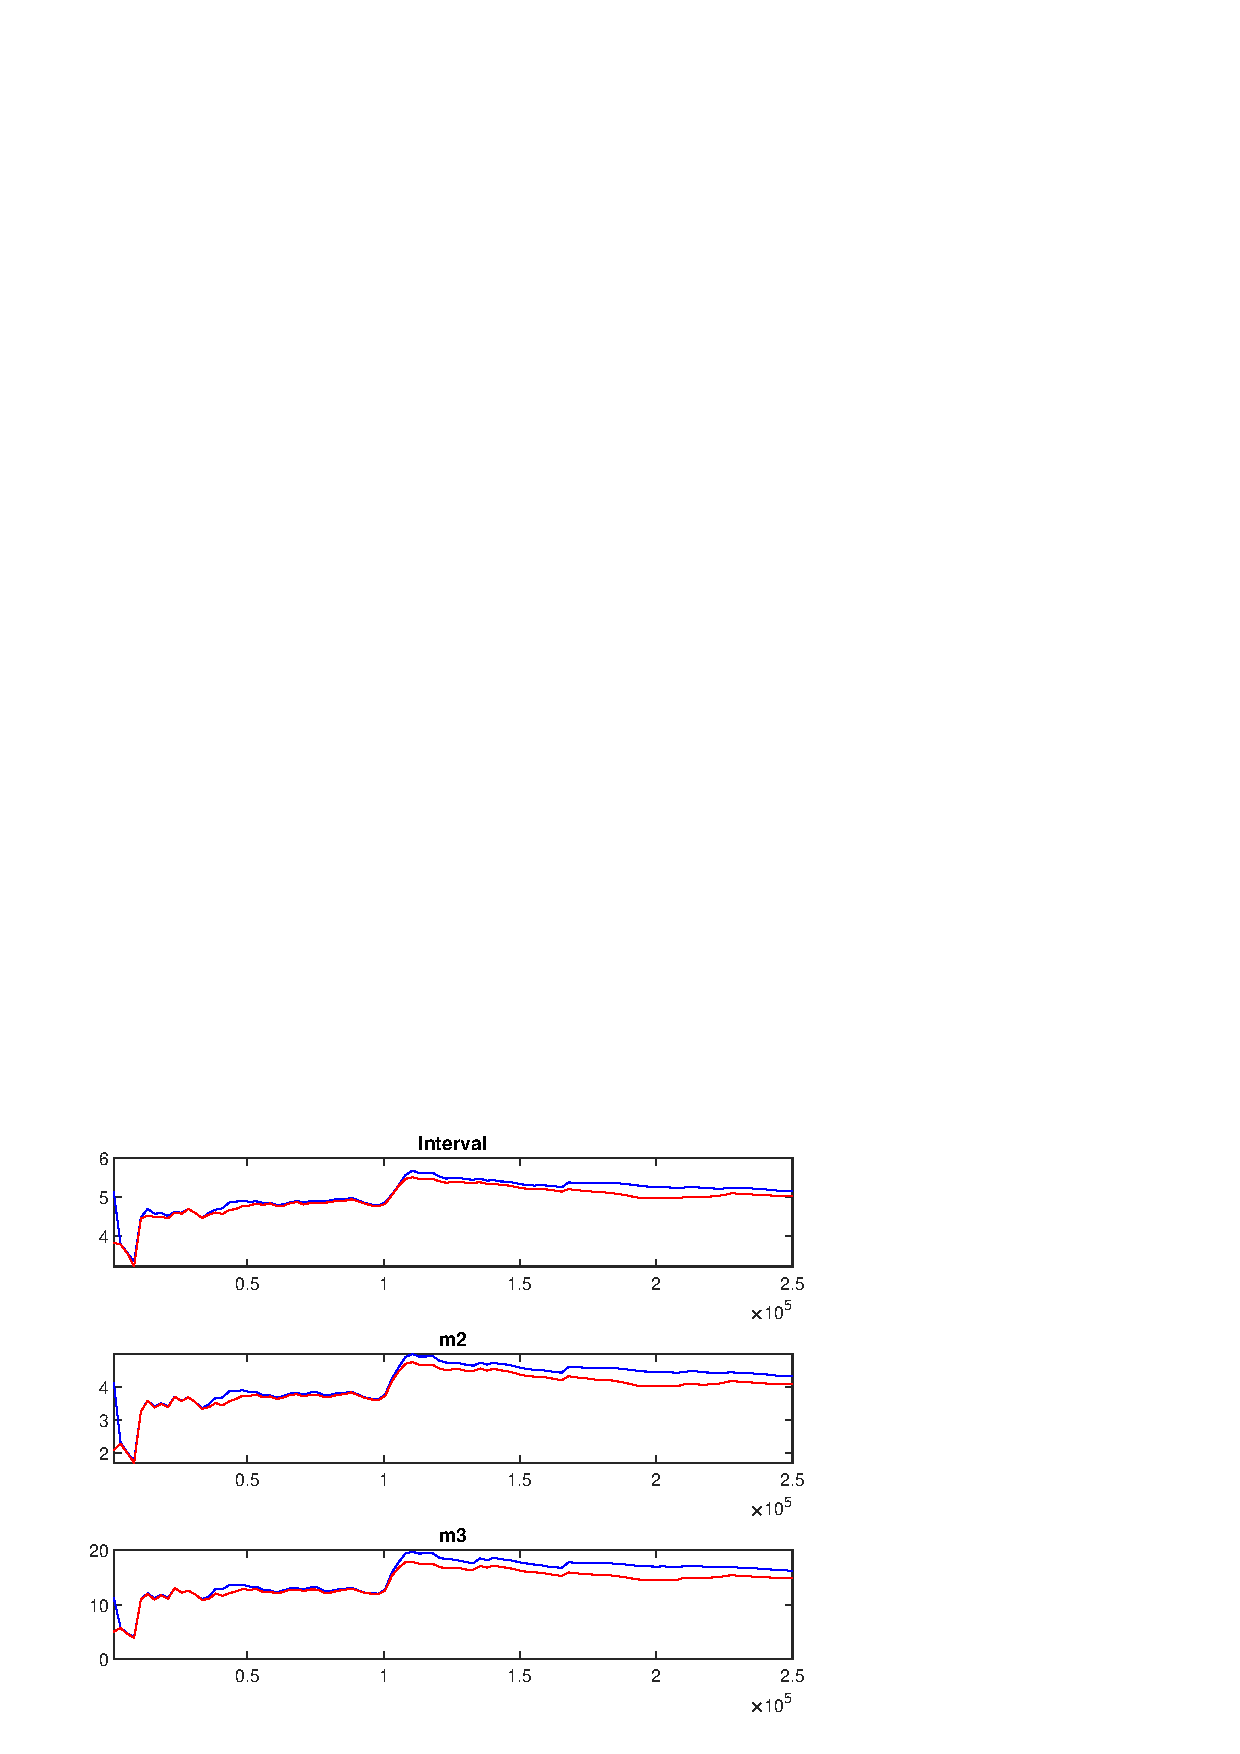
\includegraphics[width=0.8\textwidth]{BRS_util/Output/BRS_util_mdiag}
\caption{Multivariate convergence diagnostics for the Metropolis-Hastings.
The first, second and third rows are respectively the criteria based on
the eighty percent interval, the second and third moments. The different 
parameters are aggregated using the posterior kernel.}\label{Fig:MultivariateDiagnostics}
\end{figure}

% End Of TeX file. 
% TeX-table generated by Dynare.
% RESULTS FROM METROPOLIS HASTINGS (parameters)
% 30-Sep-2024 16:42:11 
 
\begin{center}
\begin{longtable}{llcccccc} 
\caption{Results from Metropolis-Hastings (parameters)}
 \label{Table:MHPosterior:1}\\
\toprule 
  & \multicolumn{3}{c}{Prior}  &  \multicolumn{4}{c}{Posterior} \\
  \cmidrule(r{.75em}){2-4} \cmidrule(r{.75em}){5-8}
  & Dist. & Mean  & Stdev. & Mean & Stdev. & HPD inf & HPD sup\\
\midrule \endfirsthead 
\caption{(continued)}\\\toprule 
  & \multicolumn{3}{c}{Prior}  &  \multicolumn{4}{c}{Posterior} \\
  \cmidrule(r{.75em}){2-4} \cmidrule(r{.75em}){5-8}
  & Dist. & Mean  & Stdev. & Mean & Stdev. & HPD inf & HPD sup\\
\midrule \endhead 
\bottomrule \multicolumn{8}{r}{(Continued on next page)} \endfoot 
\bottomrule \endlastfoot 
$(\phi)$ & beta &   0.320 & 0.2000 &   0.883& 0.0137 &  0.8628 &  0.9059 \\ 
$(\eta)$ & gamm &   0.200 & 0.1500 &   1.874& 0.0134 &  1.8575 &  1.8985 \\ 
${\rho_g}$ & beta &   0.100 & 0.0500 &   0.228& 0.0067 &  0.2199 &  0.2399 \\ 
${\rho_Z}$ & beta &   0.600 & 0.2000 &   0.972& 0.0039 &  0.9649 &  0.9770 \\ 
${\rho_{ZI}}$ & beta &   0.600 & 0.2000 &   0.999& 0.0011 &  0.9976 &  1.0000 \\ 
${\rho_N}$ & beta &   0.600 & 0.2000 &   0.979& 0.0054 &  0.9708 &  0.9883 \\ 
${\rho_D}$ & beta &   0.600 & 0.2000 &   0.928& 0.0090 &  0.9142 &  0.9408 \\ 
\end{longtable}
 \end{center}
% End of TeX file.
 
% TeX-table generated by Dynare.
% RESULTS FROM METROPOLIS HASTINGS (standard deviation of structural shocks)
% 30-Sep-2024 16:42:16 
 
\begin{center}
\begin{longtable}{llcccccc} 
\caption{Results from Metropolis-Hastings (standard deviation of structural shocks)}
 \label{Table:MHPosterior:2}\\
\toprule 
  & \multicolumn{3}{c}{Prior}  &  \multicolumn{4}{c}{Posterior} \\
  \cmidrule(r{.75em}){2-4} \cmidrule(r{.75em}){5-8}
  & Dist. & Mean  & Stdev. & Mean & Stdev. & HPD inf & HPD sup\\
\midrule \endfirsthead 
\caption{(continued)}\\\toprule 
  & \multicolumn{3}{c}{Prior}  &  \multicolumn{4}{c}{Posterior} \\
  \cmidrule(r{.75em}){2-4} \cmidrule(r{.75em}){5-8}
  & Dist. & Mean  & Stdev. & Mean & Stdev. & HPD inf & HPD sup\\
\midrule \endhead 
\bottomrule \multicolumn{8}{r}{(Continued on next page)} \endfoot 
\bottomrule \endlastfoot 
${e_g}$ & invg &   0.010 & 0.1000 &   0.017& 0.0007 &  0.0153 &  0.0177 \\ 
${e_{ZI}}$ & invg &   0.010 & 0.1000 &   0.008& 0.0004 &  0.0073 &  0.0086 \\ 
${e_Z}$ & invg &   0.010 & 0.1000 &   0.001& 0.0001 &  0.0008 &  0.0010 \\ 
${e_N}$ & invg &   0.010 & 0.1000 &   0.014& 0.0007 &  0.0127 &  0.0148 \\ 
${e_D}$ & invg &   0.010 & 0.1000 &   0.007& 0.0004 &  0.0068 &  0.0081 \\ 
\end{longtable}
 \end{center}
% End of TeX file.
 
% TeX-table generated by dynare_estimation (Dynare).
% RESULTS FROM POSTERIOR MAXIMIZATION (parameters)
% 30-Sep-2024 16:41:25 
 
\begin{center}
\begin{longtable}{llcccc} 
\caption{Results from posterior maximization (parameters)}\\
 \label{Table:Posterior:1}\\
\toprule 
  & \multicolumn{3}{c}{Prior}  &  \multicolumn{2}{c}{Posterior} \\
  \cmidrule(r{.75em}){2-4} \cmidrule(r{.75em}){5-6}
  & Dist. & Mean  & Stdev & Mode & Stdev \\ 
\midrule \endfirsthead 
\caption{(continued)}\\
 \bottomrule 
  & \multicolumn{3}{c}{Prior}  &  \multicolumn{2}{c}{Posterior} \\
  \cmidrule(r{.75em}){2-4} \cmidrule(r{.75em}){5-6}
  & Dist. & Mean  & Stdev & Mode & Stdev \\ 
\midrule \endhead 
\bottomrule \multicolumn{6}{r}{(Continued on next page)}\endfoot 
\bottomrule\endlastfoot 
$(\phi)$ & beta &   0.320 & 0.2000 &   0.8755 &     NaN \\ 
$(\eta)$ & gamm &   0.200 & 0.1500 &   1.8840 &     NaN \\ 
${\rho_g}$ & beta &   0.100 & 0.0500 &   0.2209 &     NaN \\ 
${\rho_Z}$ & beta &   0.600 & 0.2000 &   0.9709 &     NaN \\ 
${\rho_{ZI}}$ & beta &   0.600 & 0.2000 &   0.9994 &     NaN \\ 
${\rho_N}$ & beta &   0.600 & 0.2000 &   0.9816 &     NaN \\ 
${\rho_D}$ & beta &   0.600 & 0.2000 &   0.9275 &     NaN \\ 
\end{longtable}
 \end{center}
% End of TeX file.
 
% TeX-table generated by dynare_estimation (Dynare).
% RESULTS FROM POSTERIOR MAXIMIZATION (standard deviation of structural shocks)
% 30-Sep-2024 16:41:25 
 
\begin{center}
\begin{longtable}{llcccc} 
\caption{Results from posterior maximization (standard deviation of structural shocks)}\\
 \label{Table:Posterior:2}\\
\toprule 
  & \multicolumn{3}{c}{Prior}  &  \multicolumn{2}{c}{Posterior} \\
  \cmidrule(r{.75em}){2-4} \cmidrule(r{.75em}){5-6}
  & Dist. & Mean  & Stdev & Mode & Stdev \\ 
\midrule \endfirsthead 
\caption{(continued)}\\
 \bottomrule 
  & \multicolumn{3}{c}{Prior}  &  \multicolumn{2}{c}{Posterior} \\
  \cmidrule(r{.75em}){2-4} \cmidrule(r{.75em}){5-6}
  & Dist. & Mean  & Stdev & Mode & Stdev \\ 
\midrule \endhead 
\bottomrule \multicolumn{6}{r}{(Continued on next page)}\endfoot 
\bottomrule\endlastfoot 
${e_g}$ & invg &   0.010 & 0.1000 &   0.0165 &     NaN \\ 
${e_{ZI}}$ & invg &   0.010 & 0.1000 &   0.0079 &     NaN \\ 
${e_Z}$ & invg &   0.010 & 0.1000 &   0.0009 &     NaN \\ 
${e_N}$ & invg &   0.010 & 0.1000 &   0.0136 &     NaN \\ 
${e_D}$ & invg &   0.010 & 0.1000 &   0.0074 &     NaN \\ 
\end{longtable}
 \end{center}
% End of TeX file.
 
% TeX eps-loader file generated by PlotPosteriorDistributions.m (Dynare).
% 27-Jul-2025 18:14:06
 
\begin{figure}[H]
\centering
\includegraphics[width=0.80\textwidth]{SU_util/graphs/SU_util_PriorsAndPosteriors1}
\caption{Priors and posteriors.}\label{Fig:PriorsAndPosteriors:1}
\end{figure}
 
\begin{figure}[H]
\centering
\includegraphics[width=0.80\textwidth]{SU_util/graphs/SU_util_PriorsAndPosteriors2}
\caption{Priors and posteriors.}\label{Fig:PriorsAndPosteriors:2}
\end{figure}
 
% End of TeX file.
 
% TeX eps-loader file generated by mcmc_diagnostics.m (Dynare).
% 27-Jul-2025 18:13:33
 
\begin{figure}[H]
\centering 
\includegraphics[width=0.80\textwidth]{SU_util/graphs/SU_util_udiag1}
\caption{Univariate convergence diagnostics for the Metropolis-Hastings.
The first, second and third columns are respectively the criteria based on
the eighty percent interval, the second and third moments.}\label{Fig:UnivariateDiagnostics:1}
\end{figure}

\begin{figure}[H]
\centering 
\includegraphics[width=0.80\textwidth]{SU_util/graphs/SU_util_udiag2}
\caption{Univariate convergence diagnostics for the Metropolis-Hastings.
The first, second and third columns are respectively the criteria based on
the eighty percent interval, the second and third moments.}\label{Fig:UnivariateDiagnostics:2}
\end{figure}

\begin{figure}[H]
\centering 
\includegraphics[width=0.80\textwidth]{SU_util/graphs/SU_util_udiag3}
\caption{Univariate convergence diagnostics for the Metropolis-Hastings.
The first, second and third columns are respectively the criteria based on
the eighty percent interval, the second and third moments.}\label{Fig:UnivariateDiagnostics:3}
\end{figure}

\begin{figure}[H]
\centering 
\includegraphics[width=0.80\textwidth]{SU_util/graphs/SU_util_udiag4}
\caption{Univariate convergence diagnostics for the Metropolis-Hastings.
The first, second and third columns are respectively the criteria based on
the eighty percent interval, the second and third moments.}\label{Fig:UnivariateDiagnostics:4}
\end{figure}

 
% TeX eps-loader file generated by mode_check.m (Dynare).
% 27-Jul-2025 18:12:55
 
\begin{figure}[H]
\centering 
\includegraphics[width=0.80\textwidth]{SU_util/graphs/SU_util_CheckPlots1}
\caption{Check plots.}\label{Fig:CheckPlots:1}
\end{figure}
 
\begin{figure}[H]
\centering 
\includegraphics[width=0.80\textwidth]{SU_util/graphs/SU_util_CheckPlots2}
\caption{Check plots.}\label{Fig:CheckPlots:2}
\end{figure}
 
 
% TeX eps-loader file generated by dynare_estimation_1.m (Dynare).
% 27-Jul-2025 18:14:09
 
\begin{figure}[H]
\centering 
\includegraphics[width=0.80\textwidth]{SU_util/graphs/SU_util_HistoricalAndSmoothedVariables1}
\caption{Historical and smoothed variables.}\label{Fig:HistoricalAndSmoothedVariables:1}
\end{figure}


% End of TeX file.
 
% TeX eps-loader file generated by stoch_simul.m (Dynare).
% 27-Jul-2025 18:14:09
 
\begin{figure}[H]
\centering 
\includegraphics[width=0.80\textwidth]{SU_util/graphs/SU_util_IRF_e_g1}
\caption{Impulse response functions (orthogonalized shock to ${e_g}$).}\label{Fig:IRF:e_g:1}
\end{figure}
 
\begin{figure}[H]
\centering 
\includegraphics[width=0.80\textwidth]{SU_util/graphs/SU_util_IRF_e_g2}
\caption{Impulse response functions (orthogonalized shock to ${e_g}$).}\label{Fig:IRF:e_g:2}
\end{figure}
 
\begin{figure}[H]
\centering 
\includegraphics[width=0.80\textwidth]{SU_util/graphs/SU_util_IRF_e_Z1}
\caption{Impulse response functions (orthogonalized shock to ${e_Z}$).}\label{Fig:IRF:e_Z:1}
\end{figure}
 
\begin{figure}[H]
\centering 
\includegraphics[width=0.80\textwidth]{SU_util/graphs/SU_util_IRF_e_Z2}
\caption{Impulse response functions (orthogonalized shock to ${e_Z}$).}\label{Fig:IRF:e_Z:2}
\end{figure}
 
\begin{figure}[H]
\centering 
\includegraphics[width=0.80\textwidth]{SU_util/graphs/SU_util_IRF_e_ZI1}
\caption{Impulse response functions (orthogonalized shock to ${e_{ZI}}$).}\label{Fig:IRF:e_ZI:1}
\end{figure}
 
\begin{figure}[H]
\centering 
\includegraphics[width=0.80\textwidth]{SU_util/graphs/SU_util_IRF_e_ZI2}
\caption{Impulse response functions (orthogonalized shock to ${e_{ZI}}$).}\label{Fig:IRF:e_ZI:2}
\end{figure}
 
\begin{figure}[H]
\centering 
\includegraphics[width=0.80\textwidth]{SU_util/graphs/SU_util_IRF_e_N1}
\caption{Impulse response functions (orthogonalized shock to ${e_N}$).}\label{Fig:IRF:e_N:1}
\end{figure}
 
\begin{figure}[H]
\centering 
\includegraphics[width=0.80\textwidth]{SU_util/graphs/SU_util_IRF_e_N2}
\caption{Impulse response functions (orthogonalized shock to ${e_N}$).}\label{Fig:IRF:e_N:2}
\end{figure}
 
\begin{figure}[H]
\centering 
\includegraphics[width=0.80\textwidth]{SU_util/graphs/SU_util_IRF_e_D1}
\caption{Impulse response functions (orthogonalized shock to ${e_D}$).}\label{Fig:IRF:e_D:1}
\end{figure}
 
\begin{figure}[H]
\centering 
\includegraphics[width=0.80\textwidth]{SU_util/graphs/SU_util_IRF_e_D2}
\caption{Impulse response functions (orthogonalized shock to ${e_D}$).}\label{Fig:IRF:e_D:2}
\end{figure}
 
 
% End Of TeX file. 
 
% TeX eps-loader file generated by plot_priors.m (Dynare).
% 30-Sep-2024 16:41:17
 
\begin{figure}[H]
\centering
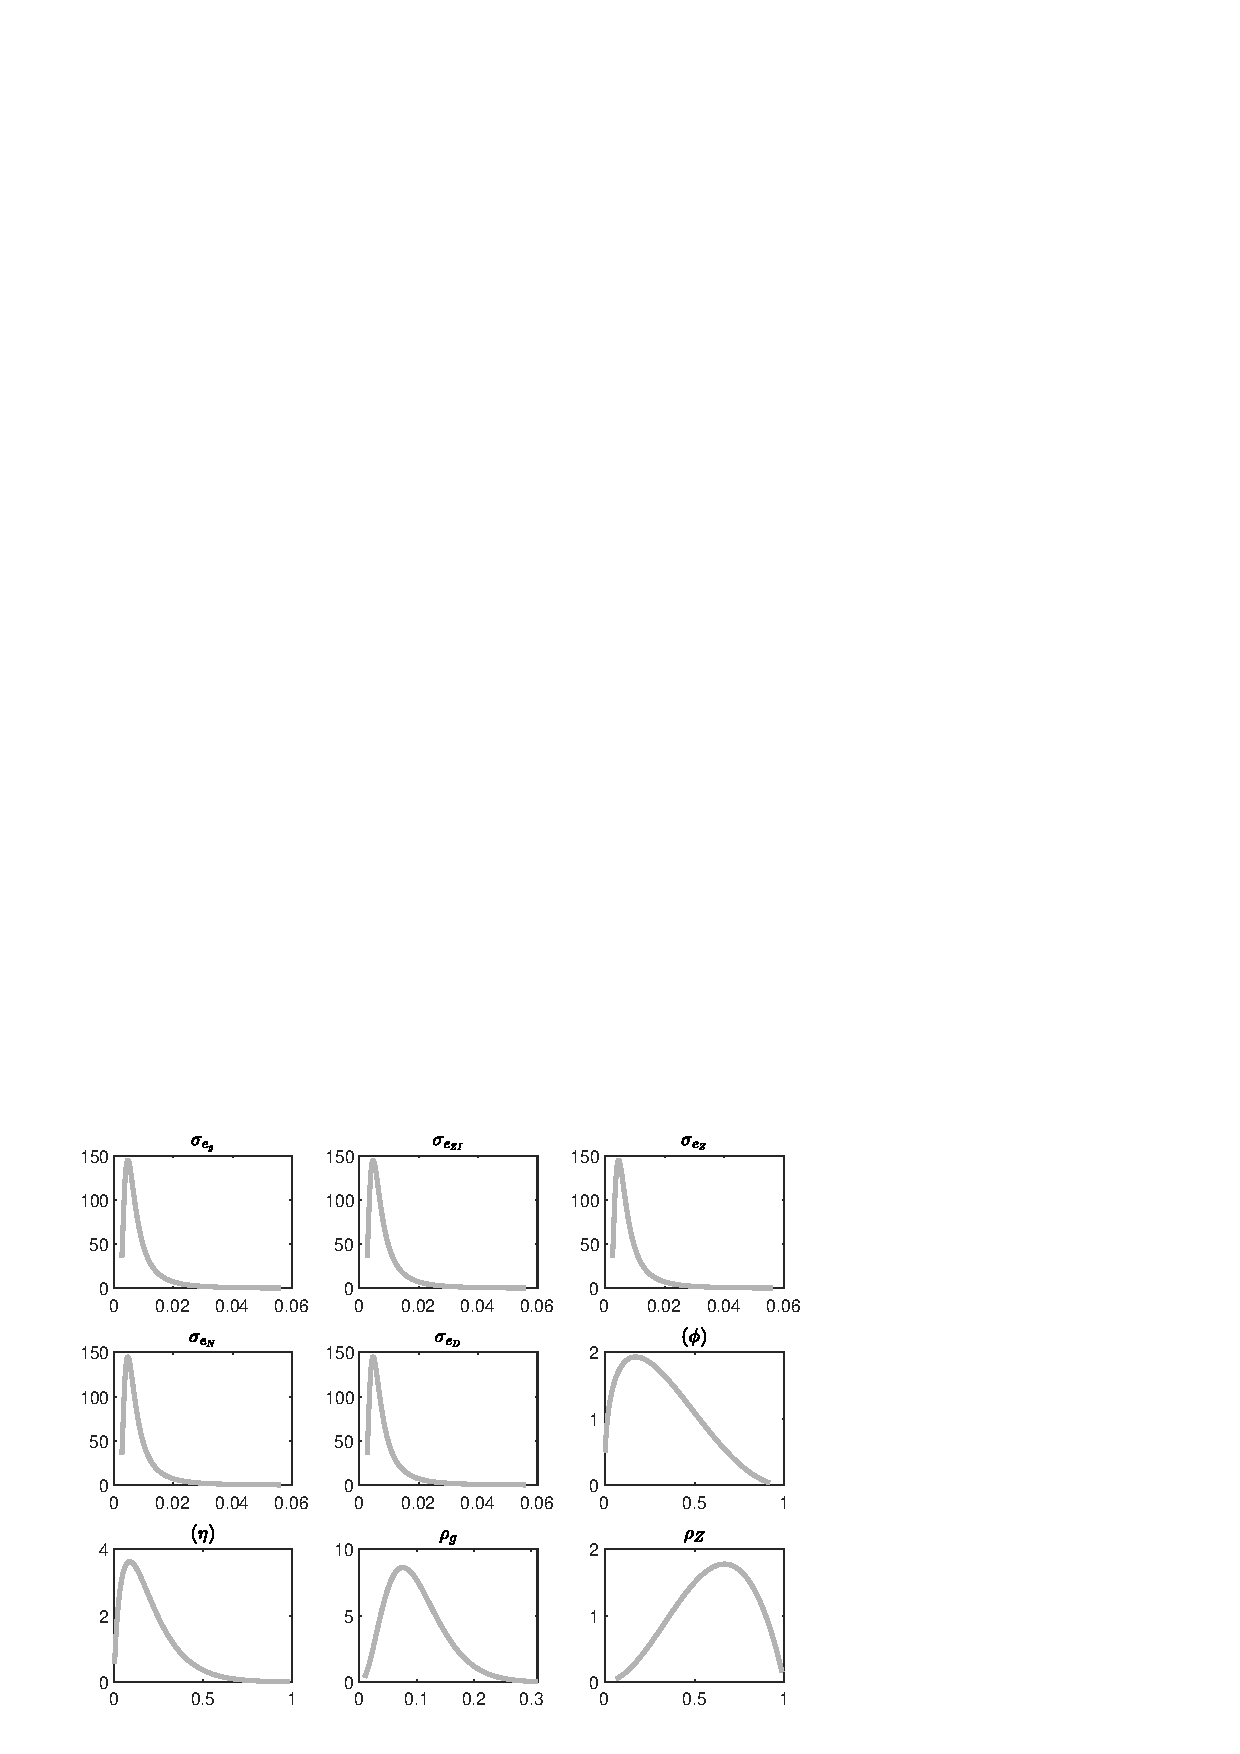
\includegraphics[width=0.80\textwidth]{BRS_util/graphs/BRS_util_Priors1}
\caption{Priors.}\label{Fig:Priors:1}
\end{figure}
\begin{figure}[H]
\centering
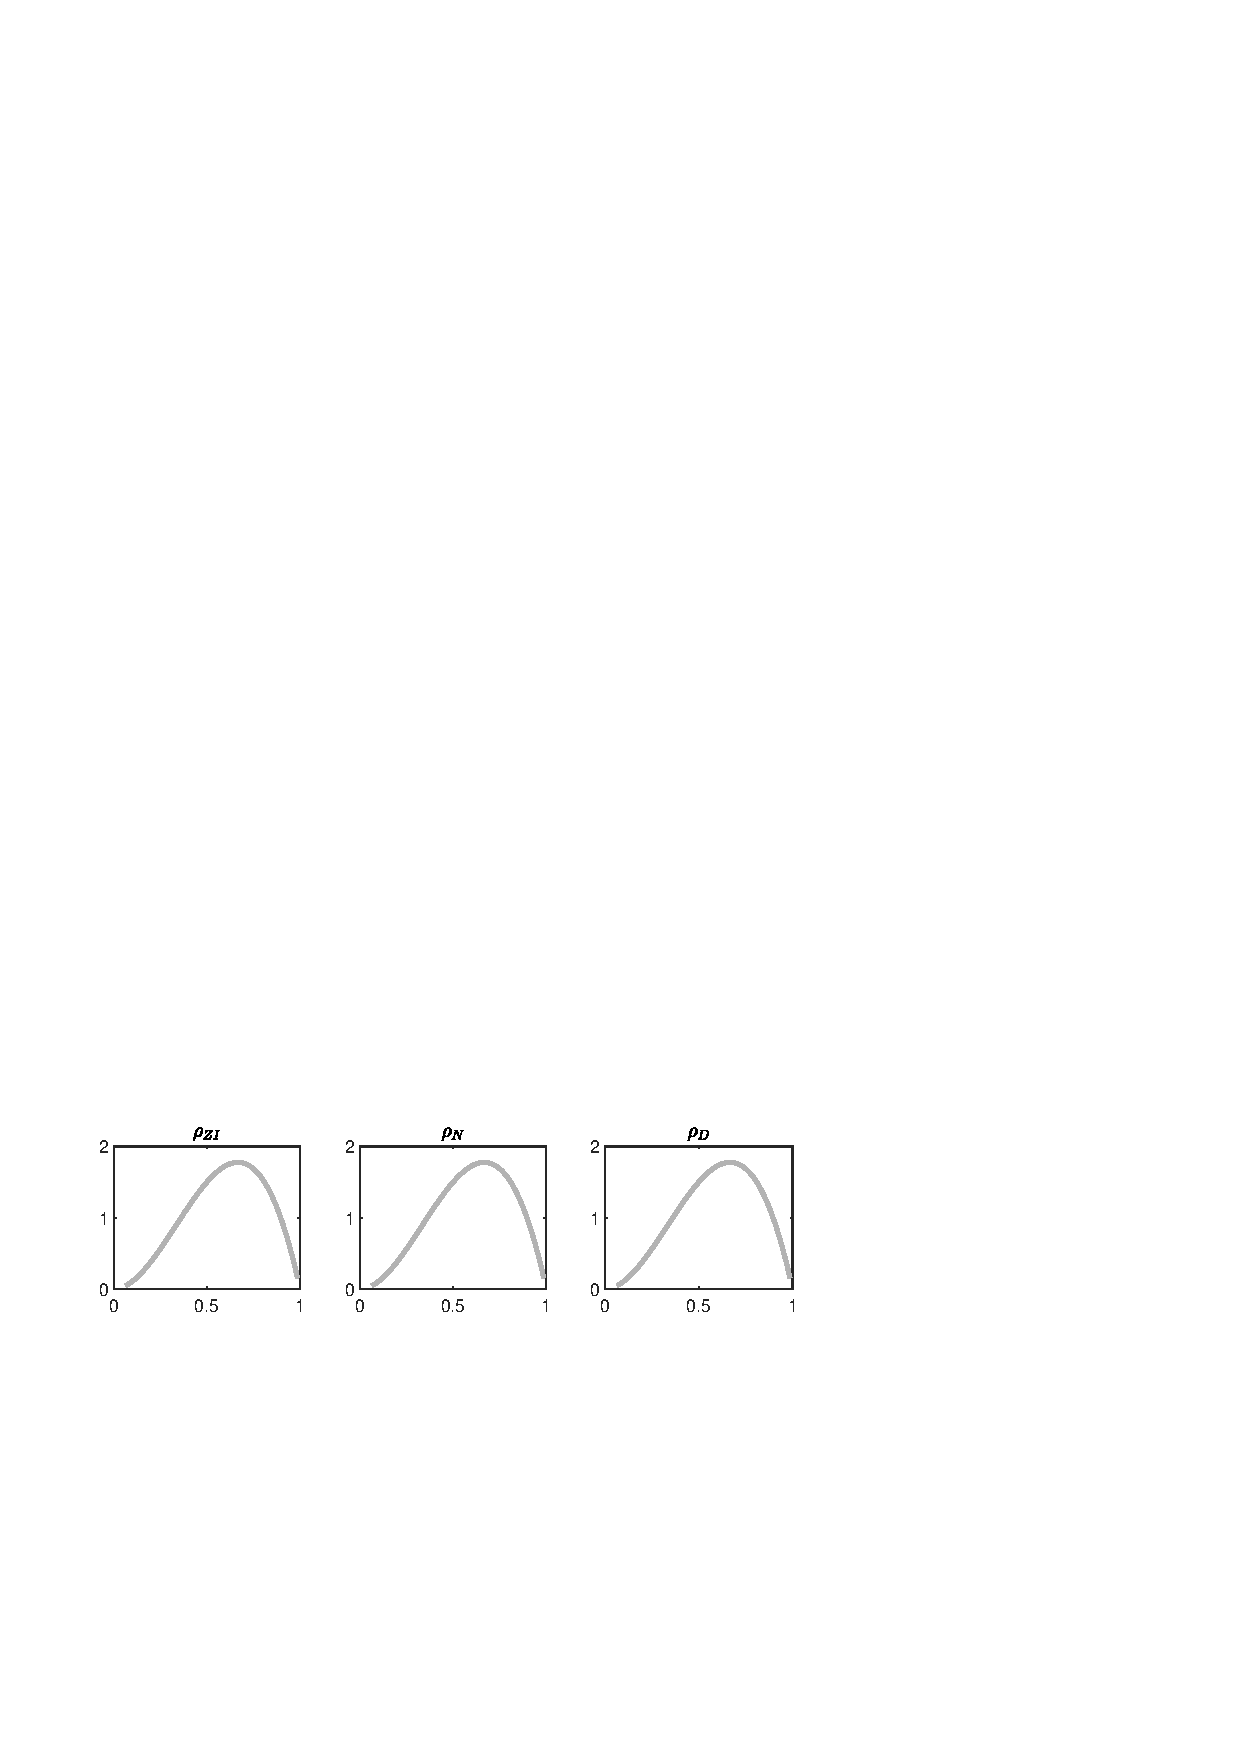
\includegraphics[width=0.80\textwidth]{BRS_util/graphs/BRS_util_Priors2}
\caption{Priors.}\label{Fig:Priors:2}
\end{figure}
 
% End of TeX file.
 
% TeX eps-loader file generated by dynare_estimation_1.m (Dynare).
% 27-Jul-2025 18:14:08
 
\begin{figure}[H]
\centering 
\includegraphics[width=0.80\textwidth]{SU_util/graphs/SU_util_SmoothedShocks1}
\caption{Smoothed shocks.}\label{Fig:SmoothedShocks:1}
\end{figure}


% End of TeX file.
 
\end{document} 
